\documentclass[12pt,oneside,reqno]{ta-its}
\usepackage{hyperref}
\usepackage{listings}
\usepackage{float}
\usepackage{mdframed}
\usepackage{wrapfig}

\renewcommand{\lstlistingname}{Kode Sumber}
\renewcommand{\lstlistlistingname}{DAFTAR KODE SUMBER}

\title{Implementasi \textit{Publish/Subscribe} pada Rancang Bangun Sistem Monitoring Perangkat Jaringan di ITS}{Implementation of Publish/Subscribe on Design of Network Monitoring Device System in ITS}{KI141502}

\author{Afif Ridho Kamal Putra}{05111440000173}

\supervisorOne{Royyana Muslim Ijtihadie S.Kom, M.Kom., Ph.D}{198407082010122004}
\supervisorTwo{Bagus Jati Santoso, S.Kom., Ph.D}{051100116}

\degree{Sarjana Komputer}{Arsitektur dan Jaringan Komputer}{S1}{Departemen Informatika}{Informatics}{Teknologi Informasi dan Komunikasi}{FTIK}{Information Technology and Communication}

\time{Juni}{2018}

\begin{document}
\renewcommand{\thelstlisting}{\arabic{chapter}.\arabic{lstlisting}}
	\frontmatter % Halaman dengan penomoran romawi kecil
	\maketitle
	\legalityPaper % Lembar Pengesahan
	
    \begin{abstrak}
		Semakin berkembangnya teknologi informasi menuntut semakin banyaknya penggunaan perangkat berupa komputer atau perangkat jaringan. Setiap perangkat jaringan memiliki fungsi masing-masing. Sebagai contoh, salah satu fungsi yang dimiliki oleh router adalah untuk medistribusikan alamat kepada tiap host agar tiap host dapat berkomunikasi satu sama lain, lalu ada pula switch yang memiliki fungsi utama yaitu menerima informasi dari berbagai sumber yang tersambung dengannya, kemudian menyalurkan informasi tersebut kepada pihak yang membutuhkannya saja.
		
		Pada suatu organisasi yang besar, kubutuhan akan perangkat jaringan sangatlah besar, terutama dalam hal jumlah perangkat yang digunakan. Banyaknya jumlah perangkat jaringan yang digunakan otomatis membuat jumlah perangkat jaringan yang dipantau juga banyak jumlahnya. Dikarenakan banyaknya jumlah perangkat jaringan yang harus dipantau, seringkali para teknisi mengalami kesulitan dalam memantau kinerja dari tiap perangkat jaringan. Oleh karena itu, dibutuhkan sebuah sistem yang dapat memantau kinerja dari setiap perangkat jaringan yang terpasang.
		
		Aplikasi yang dirancang pada tugas akhir ini, menghadirkan sebuah sistem berbasis web yang dapat memantau seluruh perangkat jaringan yang terhubung dalam jaringan dengan metode publish/subscribe, sehingga setiap user nantinya dapat memilih perangkat jaringan apa saja yang ingin dipantau, dan dapat memilih informasi apa saja yang ingin didapat kan dari tiap-tiap perangkat jaringan yang telah dipilih. \\

	\noindent \textbf{Kata-Kunci}: aplikasi web, publish/subscribe
\end{abstrak}
\newpage
\begin{abstract}
		The development of information technology requires the increasing of devices used in the form of computers or network devices. Every network device has its own function. For example, one of the functions owned by a router is to distribute the address to each host so that the host can communicate with each other, then there is also a switch that has the main function to receiving information from various sources connected to it, then channeling the information to the party who need it only.
		
		In a large organization, the need for network devices is enormous, especially in the number of devices used. The large number of network devices used, automatically keeps the number of network devices being monitored also in increased. Due to the large number of network devices to monitor, it brings technicians into a trouble to monitor the performance of each network device frequently. Therefore, a system that can monitor the performance of each installed network device is required.
		
		The application designed in this final project, presents a web-based system that can monitor all network devices connected in the network with the method of publish / subscribe, so that each user will be able to choose any network device that they want to be monitored, and can choose what information that they want to get from each network device that has been selected. \\

	\noindent \textbf{Keywords}: autoscale, docker, elastic cloud, web application
\end{abstract}
	\chapter{Kata Pengantar}
		\begin{figure}[h]
			\centering
			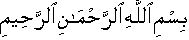
\includegraphics[width=0.5\linewidth]{img/bismillah.png}
		\end{figure}

		Alhamdulillahirabbil’alamin, segala puji bagi Allah SWT, yang telah melimpahkan rahmat dan hidayah-Nya sehingga penulis dapat menyelesaikan Tugas Akhir yang berjudul \textbf{IMPLEMENTASI PENGENDALI ELASTISITAS SUMBER DAYA BERBASIS DOCKER UNTUK APLIKASI WEB}. Pengerjaan Tugas Akhir ini merupakan suatu kesempatan yang sangat baik bagi penulis. Dengan pengerjaan Tugas Akhir ini, penulis bisa belajar lebih banyak untuk memperdalam dan meningkatkan apa yang telah didapatkan penulis selama menempuh perkuliahan di Teknik Informatika ITS. Dengan Tugas Akhir ini penulis juga dapat menghasilkan suatu implementasi dari apa yang telah penulis pelajari.
		Selesainya Tugas Akhir ini tidak lepas dari bantuan dan dukungan beberapa pihak. Sehingga pada kesempatan ini penulis mengucapkan syukur dan terima kasih kepada:
		\begin{enumerate}
			\item Allah SWT atas anugerahnya yang tidak terkira kepada penulis dan Nabi Muhammad SAW.
			\item Ibu Henning Titi Ciptaningtyas, S.Kom., M.Kom selaku pembimbing I yang telah membantu, membimbing, dan memotivasi penulis mulai dari pengerjaan proposal hingga terselesaikannya Tugas Akhir ini.
			\item Bapak Bagus Jati Santoso, S.Kom., Ph.D selaku pembimbing II yang juga telah membantu, membimbing, dan memotivasi penulis mulai dari pengerjaan proposal hingga terselesaikannya Tugas Akhir ini.
			\item Darlis Herumurti, S.Kom., M.Kom., selaku Kepala Jurusan Teknik Informatika ITS pada masa pengerjaan Tugas Akhir, Bapak Radityo Anggoro, S.Kom., M.Sc., selaku koordinator TA, dan segenap dosen Teknik Informatika yang telah memberikan ilmu dan pengalamannya.
			\item Serta semua pihak yang telah turut membantu penulis dalam menyelesaikan Tugas Akhir ini.
		\end{enumerate}

		Penulis menyadari bahwa Tugas Akhir ini masih memiliki banyak kekurangan. Sehingga dengan kerendahan hati, penulis mengharapkan kritik dan saran dari pembaca untuk perbaikan ke depannya.

		\hfill Surabaya, Juni 2017 \\ \\
		\hfill Muhammad Fahrul Razi

	\cleardoublepage % Mengisi penanda halaman genap yang kosong

	\tableofcontents % Daftar Isi
	\listoftables % Daftar Tabel
	\listoffigures % Daftar Gambar
	\lstlistoflistings % Daftar Kode Sumber

	\mainmatter
	\chapter{PENDAHULUAN}
	Pada bab ini akan dipaparkan mengenai garis besar Tugas Akhir yang meliputi latar belakang, tujuan, rumusan dan batasan permasalahan, metodologi pembuatan Tugas Akhir, dan sistematika penulisan.
        
	\section{Latar Belakang}
		Semakin berkembangnya teknologi informasi menuntut semakin banyaknya penggunaan perangkat berupa komputer atau perangkat jaringan. Setiap perangkat jaringan memiliki fungsi masing-masing. Sebagai contoh, salah satu fungsi yang dimiliki oleh router adalah untuk medistribusikan alamat kepada tiap host agar tiap host dapat berkomunikasi satu sama lain, lalu ada pula switch yang memiliki fungsi utama yaitu menerima informasi dari berbagai sumber yang tersambung dengannya, kemudian menyalurkan informasi tersebut kepada pihak yang membutuhkannya saja.
		
		Pada suatu organisasi yang besar, kubutuhan akan perangkat jaringan sangatlah besar, terutama dalam hal jumlah perangkat yang digunakan. Banyaknya jumlah perangkat jaringan yang digunakan otomatis membuat jumlah perangkat jaringan yang dipantau juga banyak jumlahnya. Dikarenakan banyaknya jumlah perangkat jaringan yang harus dipantau, seringkali para teknisi mengalami kesulitan dalam memantau kinerja dari tiap perangkat jaringan. Oleh karena itu, dibutuhkan sebuah sistem yang dapat memantau kinerja dari setiap perangkat jaringan yang terpasang.
		
		Aplikasi yang dirancang pada tugas akhir ini, menghadirkan sebuah sistem yang dapat memantau seluruh perangkat jaringan yang terhubung dalam jaringan dengan metode publish/subscribe, sehingga setiap user nantinya dapat memilih perangkat jaringan apa saja yang ingin dipantau, dan dapat memilih informasi apa saja yang ingin didapat kan dari tiap-tiap perangkat jaringan yang telah dipilih.

	\section{Rumusan Masalah}
       	Rumusan masalah yang diangkat dalam tugas akhir ini adalah sebagai berikut :
		\begin{enumerate}
			\item Bagaimana cara membuat agen polling untuk mengambil data pada suatu perangkat jaringan?
			\item Bagimana cara mengimplementasikan publish/subscribe sebagai middleware?
            \item Bagaimana cara menyaring informasi yang dipilih oleh pelanggan?
		\end{enumerate}

	\section{Batasan Masalah}
		Dari permasalahan yang telah diuraikan di atas, terdapat beberapa batasan masalah pada tugas akhir ini, yaitu:
		\begin{enumerate}
			\item User hanya dapat memonitoring perangkat jaringan (server tidak termasuk).
            \item Parameter untuk memonitor perangkat jaringan adalah ketersediaan dan beban yang ditampung.
            \item Performa yang diukur adalah response time.
		\end{enumerate}

	\section{Tujuan}
       	Tugas akhir dibuat dengan beberapa tujuan. Berikut beberapa tujuan dari pembuatan tugas akhir:
       	\begin{enumerate}
       		\item User hanya dapat memonitoring perangkat jaringan (server tidak termasuk).
       		\item Parameter untuk memonitor perangkat jaringan adalah ketersediaan dan beban yang ditampung.
       		\item Performa yang diukur adalah response time.
       	\end{enumerate}
        
	\section{Manfaat}
		Manfaat dari pembuatan tugas akhir ini antara lain adalah:
		\begin{enumerate}
			\item Memonitor ketersediaan dan beban pada sebuah perangkat jaringan.
			\item Memudahkan user untuk memonitoring perangkat jaringan yang diinginkan.
		\end{enumerate}

	\chapter{TINJAUAN PUSTAKA}
		\section{\textit{Publish/subscribe}}
			\textit{Publish/subscribe} muncul sebahai paradigma komunikasi yang populer untuk sistem terdistribusi dalam skala yang besar. dalam \textit{publish/subscribe} \textit{consumer} akan berlangganan ke suatu \textit{event} yang diinginkan. terlepas dari kegiatan \textit{consumer}, ada \textit{event producer} yang akan menerbitkan suatu \textit{event}. jika event yang diterbitkan oleh produser cocok dengan \textit{event} yang dilanggani oleh \textit{consumer}, \textit{event} tersebut akan dikirim kepada \textit{consumer} secara \textit{asynchronus}. Interaksi ini difasilitasi oleh \textit{middleware publish/subscribe}. \textit{middleware publish/subscribe} dapat dipusatkan menjadi sebuah \textit{node} tunggal yang berperan sebagai \textit{broker} dari sebuah \textit{event} atau dipisahkan menjadi kumpulan beberapa \textit{node} \textit{broker} dari sebuah \textit{event}. 
			
			pada dasarnya, \textit{publish/subscribe} dibagi dari dua jenis yaitu: \textit{topic-based} dan \textit{content-based}. Pada \textit{topic-based publish-subscribe}, \textit{event} diterbitkan melalui sebuah topik dan \textit{consumer event} akan berlangganan topik tersebut untuk mendapatkan data dari suatu \textit{event}. berlangganan pada kasus \textit{topic-based} tidak didukung pemilahan data dari suatu \textit{event}. contohnya, \textit{consumer} akan menerima semua data dari suatu \textit{event} yang diterbikan pada suatu topik. pada \textit{content-based publish-subscribe}, berlangganan pada kasus ini didukung oleh fitur pemilahan yang diterapkan pada suatu \textit{event} yang diterbitkan. data yang dipilah oleh \textit{consumer} pada suatu \textit{event} yang berlangganan akan dikirimkan ke \textit{consumer}. \cite{noauthor_what_2016}
			
		\section{\textit{Websocket}}
          	Websocket adalah protokol berbasis TCP yang menyediakan channel komunikasi full-duplex antara server dan client melalui koneksi TCP tunggal. dibandingkan dengan skema komunikasi web real-time tradisional, protokol websocket menghemat banyak sumber daya bandwidth pada jaringan, sumber daya server, dan performa real-time yang sangat jauh lebih baik dibanding websocket tradisional. Websocket adalah protocol berbasis TCP yang independen. Websocket hanya berhubungan dengan HTTP yang memiliki handshake yang diterjemahkan oleh HTTP server sebagai pengembangan dari sebuah request. Websocket terdiri dari dua bagian yaitu: handshake dan data transfer.
           		
           	Untuk membuat koneksi Websocket, client harus mengirimkan request HTTP kepada server. setelah itu protokol akan diupgrade menjadi protokol Websocket. setelah itu server akan mengenali tipe request berdasarkan header pada HTTP. Protokol akan diupgrade menjadi Websocket apalbila diminta oleh Websocket, dan kedua kubu (client dan server) akan memulai komunikasi full-duplex, yang berarti client dan server dapat bertukar data kapanpun sampai salah satu dari client atau server menutup koneksi tersebut. Model komunikasi Websocket dapat dilihat pada gambar \ref{websocketmodel}
           		
           	Websocket memiliki kemampuan yang lebih baik dalam berkomunikasi dibandingkan dengan skema komunikasi tradisional, dimana komunikasi terjadi secara realtime. sekali koneksi sudah berhasil dibuat, server dan client melakukan aliran data dua arah, dimana aktivitas tersebut meningkatkan mempuan server untuk mengirim data. Bandingkan dengan protokol HTTP, dimana informasi yang dikirimkan lebih ringkas dan mengurangi transmisi dari data yang redundan. Dengan skala user yang besar dan kebutuhan komunikasi realtime yang tinggi, menurunkan beban pada jaringan akan menjadi keuntungan dibanding komunikasi realtime secara tradisional.
           	\begin{figure}[H]
           		\centering
           		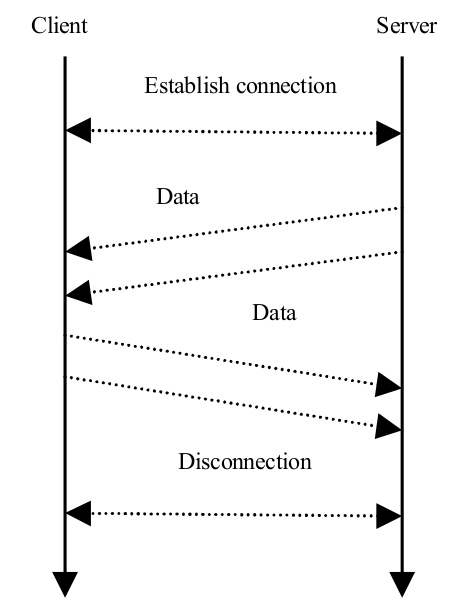
\includegraphics[height=10cm]{Images/C-2/websocket.png}
           		\caption{Model Komunikasi \textit{Websocket}}
           		\label{websocketmodel}
           	\end{figure}
           	\cite{boettiger_introduction_2015}.
		\section{SNMP}
			Simple Network Management Protocol (SNMP) adalah aplikasi pada layer protokol yang digunakan untuk mengatur data pada jaringan. hampir semua vendor jaringan mendukung protokol SNMP. beberapa vendor peralatan telekomunikasi juga mulai didukung oleh protokol SNMP untuk mencapai pengaturan (manajemen) yang terintegrasi. Banyak dari aktivitas manajemen jaringan pada jaringan enterprise yang menggunakan SNMP dalam persentasi yang sangat besar.
			
			SNMP yang berdasarkan paradigma server - client termasuk kedalam manajemen stasiun, agen dan Management Information Bases (MIB). tujuan dari manajemen stasiun adalah untuk mengirimkan request kepada agent dan mengendalikan mereka, manajemen stasiun juga menyediakan antarmuka antara manajer jaringan manusia dan sistem manajemen jaringan. setiap perangkat jaringan memungkinkan untuk mempunyai agen yang dapat mengendalikan basis data dan ketika stasiun manajemen mulai melakukan polling, agen-agen tersebut akan mengirimkan laporan kepada stasiun manajemen.
			
			Dalam pendekatan pemantauan dengan menggunakan SNMP, setiap agen akan mengirimkan stasiun manajemen sebuah informasi melalui polling laporan kejadian. Polling adalah aktivitas untuk melakukan interaksi antara agen dan stasiun manajemen menggunakan metode request dan response. Namun, stasiun manajemen hanya mendengarkan kepada informasi masuk pada pendekatan pelaporan kejadian. Agen akan mengirim informasi kepada stasiun manajemen setiap informasi tersebut dibutuhkan berdasarkan sebuah keputusan.
			
			Pendekatan pemantauan seacar realtime akan didefinisikan sebagai persetujuan antara agen dan stasiun manajemen dimana pada persetujuan semacam in agen harus mengirimkan informasi kepada manajemennya secara berkala tanpa permintaan dari stasiun.
			
			Dalam sebuah kelompak, status dan sifat dari sistem akan dipertimbangkan sebagai pekerjaan memantau dari informasi MIB. tipe data yang akan digunakan untuk memantau lebih penting dibandingkan dengan perancangan jaringan. berikut ini adalah ingormasi yang harus digunakan dalah pemantauan:
			\begin{itemize}
				\item Static: Struktur dan elemen didalam konfigurasi dikategorikan seperti id dari port pada sebuah router atau host. Informasi ini akan jarang berubah.
				\item Dynamic: Informasi kejadian pada jaringan seperti paket dan elemen jaringan
				\item Statistical: Informasi harus berasal dari informasi dinamis seperti rata-rata dari paket yang dikirimkan pada tiap unit.
			\end{itemize}
		\subsection{OID}
			Object Identifier adalah sesuatu untuk mengidentifikasi sebuah objek. Objek ini dapat berupa daerah atau disk drive tunggal. Yang paling umum, didalam IEEE-RAC, adalah OUI (Organizationally Unique Identifier), dan diturunkan secara terorganisasir, dan terdaftar diluar OUI. pengidentifikasi yang paling umum selanjutnya, termasuk pengidentifikasi alamat ethernet adalah pengidentifikasi Extended Unique Identifiers (EUI) atau the World Wide Name (WWN). uniknya, untuk sistem yang sesuai, merupakan properti berharga dalam dua kasus ini. keunikan ini diasumsikan oleh struktur dari nomor unik yang dimulai dengan OUI. IEEE-RAC menetapkan OUI sebagai Object Identifier untuk sebuah organisasi. Object Identifier ini merupakan lapisan didalam konteks yang lebih luas dari pengidentifikasi yang diturunkan secara unik dari titik awal dari sebuah OID, International
			Telecommunication Union Telecommunication Standardization Sector (ITU-T) dan dideskripsikan didalam standar ASN.1. jalur tersebut dilacak menuju ITU-T disebut sebagai "arc" dari sebuah OID. arc ini berkembang menjadi OUI dan RAC lain menetapkan perancang dan melalui penempatan yang dibuat oleh organisasi hingga titik akhir dari sebuah Object Identifier.
			\begin{figure}[H]
				\centering
				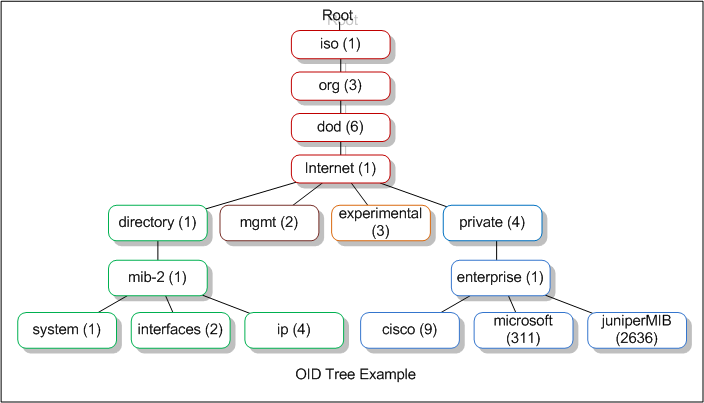
\includegraphics[width=10cm]{Images/C-2/OID.png}
				\caption{Contoh \textit{Object Identifier} (OID)}
				\label{oidexample}
			\end{figure}
		\section{Nagios}
			Nagios adalah perangkat lunak opensource yang aktif dikembangkan, memiliki banyak user juga komunitas yang luas, memiliki banyak plugin tambahan yang dikembangkan oleh user maupun yang terdapat langsung pada awal pengaturan, dan banyak buku tentang Nagios yang diterbitkan. Nagios juga merupakan sistem pemantauan yang paling yang paling populer yang cocok dengan hampir semua distribusi linux. Dukungan komersial tersedia dari perusahaan yang didirikan oleh penciptanya dan pengembang utama sebagai penyedia solusi resmi. Peralatan pemantauan yang berbasis nagios juga tersedia, seperti sensor yang dirancang untuk beroprasi bersama nagios. Karena fleksibilitas dari rancangan perangkat lunak yang menggunakan arsitektur plug-in, layanan pengecekan untuk aplikasi yang pustakanya sudah ditentukan dapat di gunakan. didalam nagios terdapat beberapa plugin lain, seperti script tambahan yang dapat dikostumisasi dan dapat digunakan pada nagios. Nagios adalah program yang ringan dan menyediakan alat pemantauan yang sempurna yang dapat membantu untuk memantau seluruh protokol yang aktif dan perakngkat jaringan yang terhubung dengan topologi. Nagios juga mampu untuk menyediakan grafik yang komperhensif dan bersifat realtime dan analisis tren.
			
		\section{REST API}
			
	\chapter{DESAIN DAN PERANCANGAN}
    Pada bab ini dibahas mengenai analisis dan perancangan sistem.
	
    \section{Kasus Penggunaan}
    	Terdapat dua aktor dalam sistem ini, yaitu Pengembang (Administrator) dan \textit{User} (Pengguna) dari aplikasi web yang dikelola oleh sistem. Diagram kasus penggunaan digambarkan pada Gambar \ref{usecase}.
        \begin{figure}[H]
			\centering
			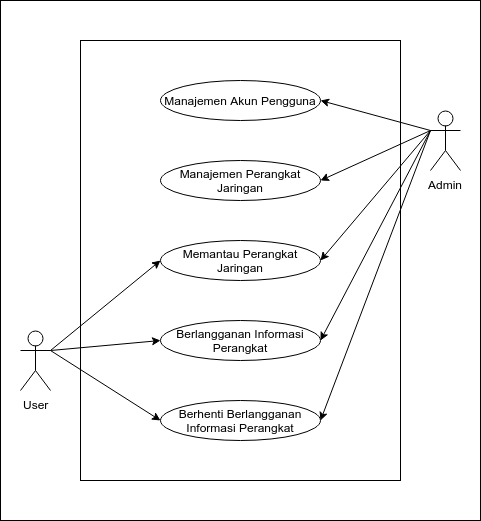
\includegraphics[width=8cm,height=10cm]{Images/C-3/usecase.png}
			\caption{Diagram Kasus Penggunaan}
			\label{usecase}
		\end{figure}
        \indent Diagram kasus penggunaan pada Gambar \ref{usecase} dideskripsikan masing-masing pada Tabel \ref {tabelKodeKasusPenggunaan}.
        
        \begin{longtable}{|p{0.25\textwidth}|p{0.24\textwidth}|p{0.35\textwidth}|} % L = Rata kiri untuk setiap kolom, | = garis batas vertikal.
		    	
		    	% Kepala tabel, berulang di setiap halaman
		    	\caption{Daftar Kode Kasus Penggunaan} \label{tabelKodeKasusPenggunaan} \\
		    	\hline
		    	\textbf{Kode Kasus Penggunaan} & \textbf{Nama Kasus Penggunaan} & \textbf{Keterangan} \\ \hline
		    	\endhead
		    	\endfoot
		    	\endlastfoot
		    	UC-0001 & Manajemen Akun Pengguna. & Pengembang (Admin) dapat membuat, melihat, mengubah dan menghapus data akun pengguna. \\ \hline
		    	UC-0002 & Manajemen Perangkat Jaringan.  & Pengembang (Admin) dapat membuat, melihat, mengubah dan menghapus data perangkat jaringan.\\ \hline
		    	UC-0003 & Memantau Perangkat Jaringan. & Pengembang (Admin) dan Pengguna (User) dapat memantau seluruh perangkat jaringan yang sudah ia langgani. \\ \hline
		    	UC-0004 & Berlangganan Informasi Perangkat. & Pengembang (Admin) dan Pengguna (User) dapat berlangganan informasi perangkat jaringan yang diinginkan. \\ \hline
		    	UC-0005 & Berhenti Berlangganan Informasi Perangkat. & Pengembang (Admin) dan Pengguna (User) dapat berhenti berlangganan informasi perangkat jaringan yang diinginkan. \\ \hline	
		    \end{longtable}

	\section{Arsitektur Sistem}
		Pada sub-bab ini, dibahas mengenai tahap analisis dan kebutuhan bisnis dan desain dari sistem yang akan dibangun.

		\subsection{Desain Umum Sistem}
			Sistem yang akan dibuat yaitu sistem yang dapat melakukan pemantauan pada perangkat jaringan yang berbasis \textit{web} dengan metode \textit{pusblish/subscribe}, dimana pengguna (\textit{user}) harus berlangganan kepada suatu informasi untuk mendapatkan informasi yang diinginkan.
			
			Sistem ini melibatkan 3 (Tiga) server yang berfungsi sebagai web server dan 1 (satu) server yang berfungsi sebagai database server. Server aplikasi dan websocket server berada pada satu server, sehingga pada implementasinya webserver aplikasi dan websocket dijalankan pada port yang berbeda. Pada sistem ini \textit{client} yaitu pengguna (\textit{user}) dan pengelola (\textit{admin}) akan mengakses aplikasi menggunakan web browser. yang nantinya jika mengakses fitur selain memantau perangkat jaringan, aplikasi akan mengirimkan \textit{request} HTTP kepada REST API, dimana REST API tersebut melakukan transaksi data kepada database server. setelah itu REST API akan mengirimkan \textit{response} kepada aplikasi.
			
			jika client mengakses fitur memantau jaringan, maka aplikasi akan terhubung dengan websocket yang tugasnya mengakses data yang berada pada pub/sub server, dimana pubsub server menyimpan data yang diterbitkan oleh nagios, data tersebut adalah hasil response SNMP nagios kepada tiap perangkat jaringan terkait.
			Penjelasan secara umum arsitektur sistem akan diuraikan pada Gambar \ref{DesainUmumSistem}.
            \begin{figure}[H]
				\centering
				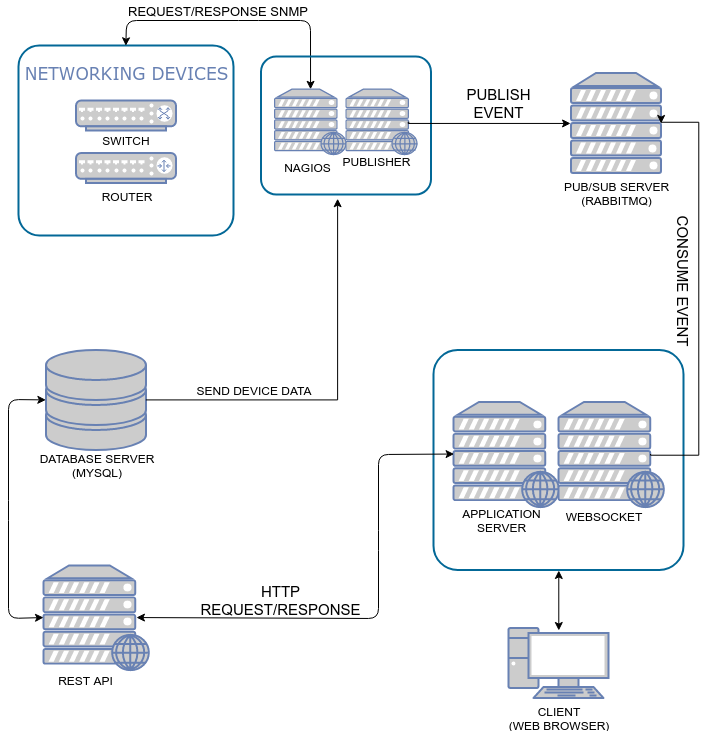
\includegraphics[width=9cm,height=8cm]{Images/C-3/main.png}
				\caption{Desain Umum Sistem}
				\label{DesainUmumSistem}
			\end{figure}

		\subsection{Desain REST API}
            	REST API bertujuan untuk menjadikan sistem yang memiliki performa yang baik, cepat dan mudah untuk di kembangkan (scaleable) terutama dalam pertukaran dan komunikasi data. REST API diakses menggunakan protokol HTTP. Penamaan dan struktur URL yang konsisten akan menghasilkan API yang baik dan mudah untuk dimengerti developer. URL API biasa disebut endpoint dalam pemanggilannya.
            	
            	Pada sistem ini terdapat beberapa endpoint, beberapa endpoint dibagi menjadi beberapa endpoint sesuai dengan perintah yang diajalankannya. misal: create, read, delete, update dan lain-lain.
            	
            	Server aplikasi mengirimkan HTTP request kepada REST API yang nantinya REST API akan melakukan trasaksi data pada database sesuai dengan endpointnya masing-masing. setelah itu REST API akan mengirimkan HTTP response kepada server aplikasi.
            	
            	Secara umum, arsitektur dari REST API dapat dilihat pada Gambar \ref{desain:desainrestapi}\\
                \begin{figure}[H]
                    \centering
                    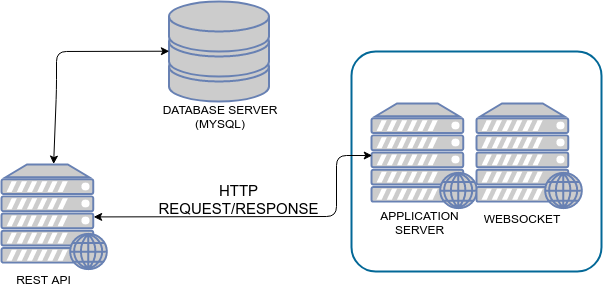
\includegraphics[width=9cm]{Images/C-3/desainrestapi.png}
                    \caption{Desain REST API}
                    \label{desain:desainrestapi}
				\end{figure}
            
		\subsection{Desain Publisher Server}
			Pada publisher server, dipasang aplikasi untuk memantau kinerja jaringan, yaitu Nagios. Pada nagios, perdapat plugin untuk memantau kinerja jaringan dengan protokol SNMP yaitu check-snmp. plugin ini membutuhkan beberapa parameter, diantaranya: alamat perangkat yang ingin dipantau dan oid dari apa yang ingin dipantau.
			
			Sebuah script dibuat untuk mengambil data dan mengirimkannya menuju pub/sub server. setiap perangkat yang dipantau dimasukkan ke sebuah thread baru agar dapat berjalan secara paralel. didalam thread tersebut, setiap perangkat terkait diperiksa kinerjanya dengan protokol SNMP dan hasilnya dikirimkan kepada pub/sub server melalui sebuah exchange yang telah diikat dengan sebuah message queue yang sebelumnya telah diinisiasi. Rancangan umum dari \textit{Publisher Server} seperti yang digambarkan pada Gambar \ref{desain:desainpublisher}.
			
			Exchange yang dibuat oleh script tersebut namanya dibuat berdasarkan uuid versi 4 dari tiap device yang diambil dari database dan nama queue dibuat berdasarkan uuid versi 4 yang dibuat baru.
			
			\begin{figure}[H]
				\centering
				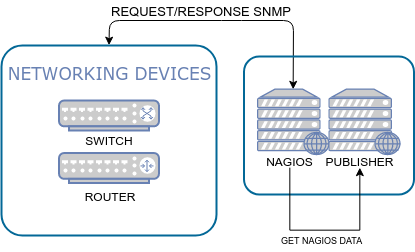
\includegraphics[width=9cm]{Images/C-3/desainpublisher.png}
				\caption{Desain Publisher Server}
				\label{desain:desainpublisher}
			\end{figure}
                
		\subsection{Desain Pub/Sub Server}
			Publish/subscribe server atau bisa juga disebut pub/sub server. yaitu sebuah server untuk menampung seluruh pesan yang dikirimkan oleh publisher. didalamnya terpasang aplikasi message broker yaitu \texttt{RabbitMQ}. seluruh pesan yang dikirimkan oleh publisher dikirimkan ke pub/sub server melalui sebuah exchange yang diikat dengan sebuah queue setelah itu server akan menyimpan pesan queue tersebut hingga ada consumer yang meminta data tersebut untuk dikirimkan. dalam kasus ini yang bertindak sebagai consumer adalah websocket server.
			
			Di sisi websocket dan server aplikasi, websocket menginisiasi sebuah exchange yang namanya dibuat berdasarkan uuid versi 4 dari tiap perangkat yang ingin dipantau dari database server, dengan syarat exchange dengan nama tersebut belum dibuat atau terdaftar sebelumnya. jika exchange dengan nama tersebut sudah dibuat atau terdaftar sebelumnya pada pub/sub server maka websocket server tidak perlu membuat exchange tersebut.
			
			Begitu juga dengan queue-nya. queue dibuat dengan nama uuid yang telah dibuat acak oleh client dengan algoritma uuid versi 4, dengan syarat queue dengan nama tersebut belum dibuat atau terdaftar sebelumnya. Jika queue dengan nama tersebut sudah dibuat atau terdaftar sebelumnya pada pub/sub server maka websocket server tidak perlu membuat queue tersebut.
			
	 		Setelah menghadapi masalah pembuatan exchange dan queue, websocket baru mengambil data perangkat pada pub/sub server sesuai dengan data apa saja yang dilanggani oleh client.
	 		
        	Secara umum, arsitektur rancangan dari \textit{Pub/Sub Server} dapat dilihat pada Gambar \ref{desain:desainpubsub}.
        	\begin{figure}[H]
				\centering
				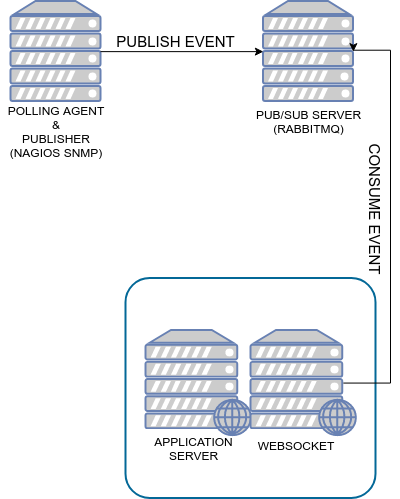
\includegraphics[width=7cm,height=7cm]{Images/C-3/desainpubsub.png}
				\caption{Desain Pub/Sub Server}
				\label{desain:desainpubsub}
			\end{figure}
		
		\subsection{Desain Consumer pada Application Server dan Websocket}
			Consumer berfungsi untuk mengambil data yang dibutuhkan oleh client dari pub/sub server. Pada sistem ini, consumer didesain untuk diimplementasikan pada websocket agar data yang diterima oleh client adalah data yang paling terbaru (realtime). websocket ini nantinya akan disambungkan dengan sebuah endpoint (URL) pada aplikasi.
			
			Consumer ini nantinya akan membuat sebuah queue dengan nama yang ditentukan oleh client. nama dari queue tersebut ditentukan dengan membuat string UUID versi 4 secara acak. Setelah berhasil membuat queue, consumer membuat exchange yang banyaknya sejumlah perangkat yang terdaftar pada sistem dan exchange tersebut diberi nama sesuai dengan ID pada masing-masing perangkat yang dimana ID tersebut berformat UUID versi 4. Pembuatan queue dan exchange akan dilakukan jika queue dan exchange belum terdaftar pada pub/sub server. jika queue dan exchange sudah terdaftar, maka tidak akan ada queue dan exchange yang akan dibuat. Setelah queue dan exchange berhasil dibuat. queue tersebut akan diikat dengan satu atau lebih exchange. lewat queue tersebutlah data akan dikirim. ilustrasi cara kerja queue dan exchange dapat dilihat pada gambar \ref{desain:consumer}.
			\begin{figure}[H]
				\centering
				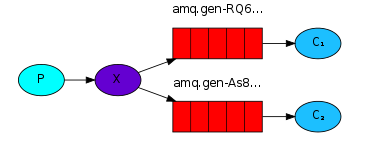
\includegraphics[height=3cm]{Images/C-3/pubsubillus.png}
				\caption{Ilustrasi Cara Kerja Queue dan Exchange}
				\label{desain:consumer}
			\end{figure}

        \subsection{Desain Database Server}        	
        	Desain database pada sistem ini adalah seperti yang digambarkan pada gambar \ref{desain:desaindatabase}. Terdapat tiga tabel utama yang mewakili tiap entitas yang terlibat dalam sistem ini, yaitu: users, devices, dan oid. selain itu, terdapat dua table many-to-many untuk menyimpan data pengguna yang telah berlangganan kepada tiap perangkat dan pengguna yang berlangganan kepada tiap OID (untuk mengetahui informasi apa saja yang ada pada tiap perangkat. tiap OID memiliki informasi yang berbeda).
        	
        	\begin{figure}[H]
        		\centering
        		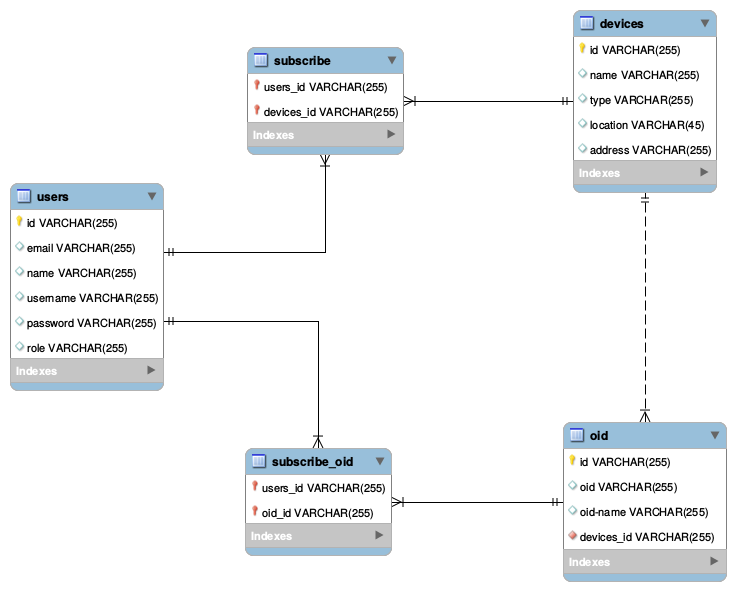
\includegraphics[width=9cm]{Images/C-3/desaindb.png}
        		\caption{Desain Database}
        		\label{desain:desaindatabase}
        	\end{figure}
        	
		\subsection{Desain Antarmuka}
			Desain antarmuka adalah desain untuk halaman yang nantinya akan digunakan oleh client baik itu pengguna (user) ataupun pengelola (admin). Antarmuka yang nantinya dibuat berbasis web dan  menggunakan Bootstrap 3 dan HTML. terdapat beberapa perbedaan pada antarmuka yang digunakan oleh pengelola dan pengguna. Misal, pada antarmuka yang digunakan pengguna tidak ada tombol untuk menghapus data perangkat, sedangkan pada antarmuka yang digunakan oleh pengelola terdapat tombol untuk menghapus data perangkat yang telah terdaftar.
			
			Desain antarmuka untuk menampilkan daftar seluruh perangkat yang tersedia pada sistem dapat dilihat pada gambar \ref{desain:antarmuka1}. pada halaman ini pengguna dan pengelola dapat meliahat daftar perangkat yang tersedia dan beberapa infonya, seperti: nama perangkat, alamat, dan lokasi dari perangkat tersebut. pada halaman in ipengguna dan pengolola juga bisa langsung berlangganan atau berhenti berlangganan dengan menekan sebuah tombol yang ada pada halaman ini.
        	\begin{figure}[H]
        		\centering
        		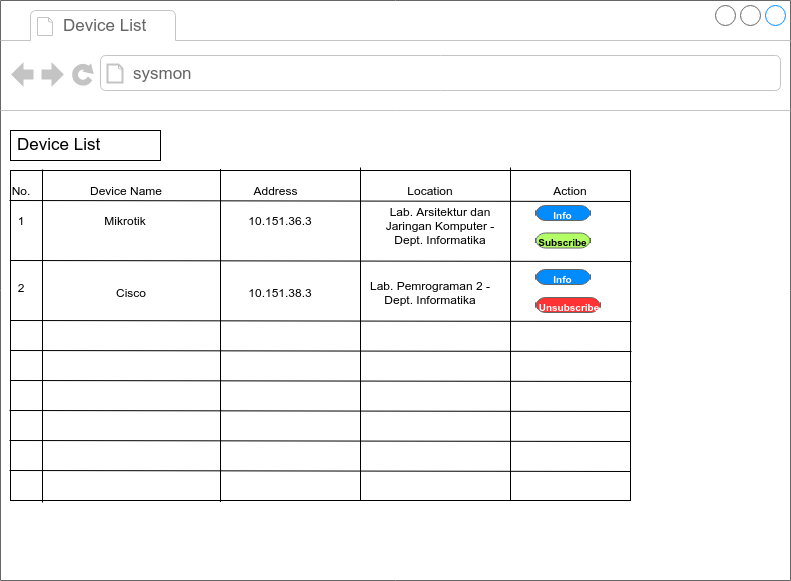
\includegraphics[width=9cm]{Images/C-3/antarmuka1.png}
        		\caption{Desain Antarmuka Menampilkan Daftar Perangkat Yang Tersedia}
        		\label{desain:antarmuka1}
        	\end{figure}
        
        	Desain antarmuka untuk menampilkan rincian dari antarmuka terkait dapat dilihat pada gambar \ref{desain:antarmuka2}. pada halaman ini pengguna dan pengolola dapat melihat seluruh rincian data yang ada pada perangkat. mulai dari nama perangkat, tipe perangkat, alamat perangkat, lokasi perangkat dan info apa saja yang dapat dipantau memalui OID.
        	
        	Pada halaman ini pengguna dan pengelola juga dapat belangganan dengan cara menekan sebuah tombol. tidak hanya berlangganan perangkatnya saja, pengguna dan pengelola juga dapat memilih untuk berlangganan info apa saja yang ingin didapatkan dari perangkat tersebut.
	        \begin{figure}[H]
	        	\centering
	        	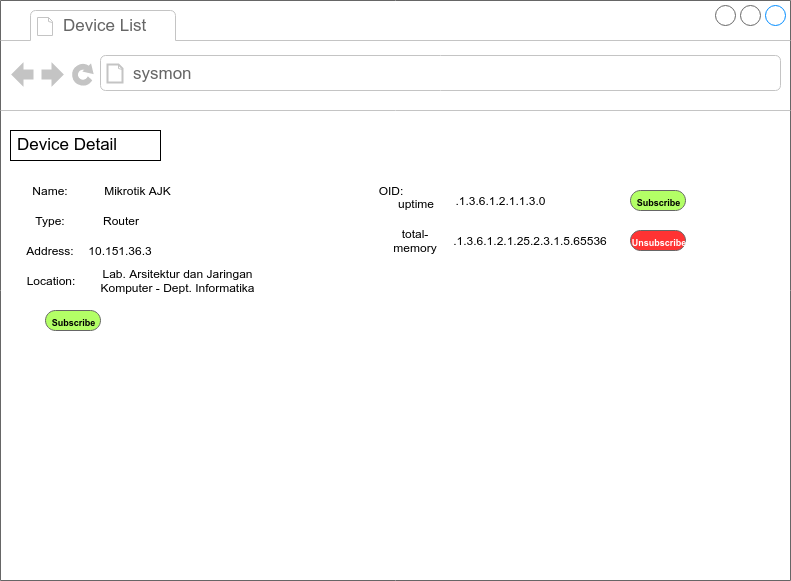
\includegraphics[width=9cm]{Images/C-3/antarmuka2.png}
	        	\caption{Desain Antarmuka Menampilkan Rincian dari Perangkat Terkait}
	        	\label{desain:antarmuka2}
	        \end{figure}
        
	        \begin{figure}[H]
	        	\centering
	        	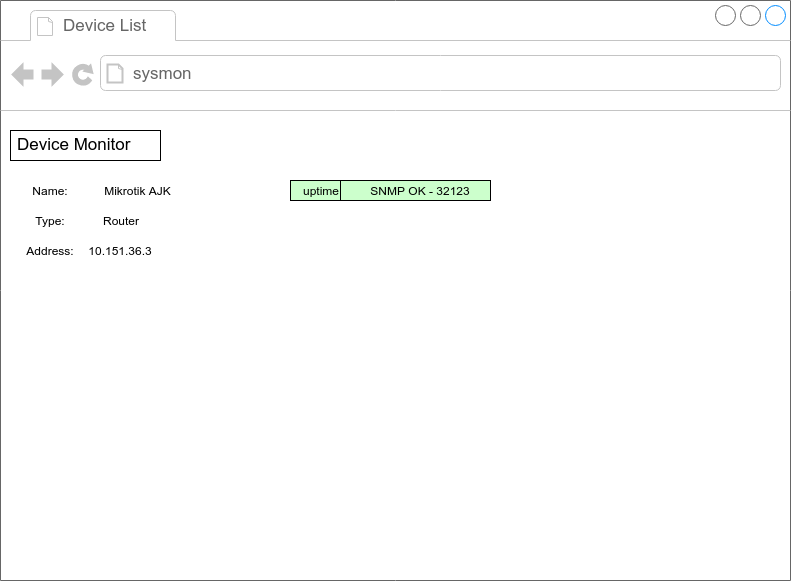
\includegraphics[width=9cm]{Images/C-3/antarmuka3.png}
	        	\caption{Desain Antarmuka Pemantauan Perangkat}
	        	\label{desain:antarmuka3}
	        \end{figure}
        
        	Desain antamuka pemantauan pernangkat dapat dilihat pada gambar \ref{desain:antarmuka3}. pada halaman ini, pengguna dan pengelola akan mendapatkan data dari seluruh perangkat yang sudah dilanggani. data yang ditampilkan pada halaman ini dipilih berdasarkan info yang dipilih pada antarmuka menampilkan rincian dari antarmuka terkait yang bisa dilihat pada gambar \ref{desain:antarmuka2}.

	\chapter{IMPLEMENTASI}
	Bab ini membahas implementasi sistem pemantauan perangkat jaringan secara rinci. Pembahasan dilakukan secara rinci untuk setiap komponen yang ada, yaitu: REST API, Publisher server, Pub/sub Server, Server aplikasi dan websocket, Database server dan Antarmuka.
    
    \section{Lingkungan Implementasi}
    	Lingkungan implementasi dan pengembangan dilakukan menggunakan virtualisasi Proxmox dengan spesifikasi \textit{Host} komputer adalah Intel(R) Core(TM) i3-2120 CPU @ 3.30GHz dengan memori 8 GB di Laboratorium Arsitektur dan Jaringan Komputer, Teknik Informatika ITS. Perangkat lunak yang digunakan dalam pengembangan adalah sebagai berikut:
        \begin{itemize}
        \item Sistem Operasi Linux Ubuntu Server 16.04 LTS
        \item RabbitMQ 3.7.5-1
        \item MySQL Ver 15.1 Distrib 10.0.34-MariaDB
        \item Python 2.7
        \item Flask 0.12.2
        \item Node.js v6.11.4
        \item Nagios 4.3.4
        \item Express.js 4.16.3
        \end{itemize}
        
	\section{Implementasi REST API}
    	REST API digunakan untuk memudahkan aplikasi agar ringan dan mudah untuk dikembangkan. pada tugas akhir ini, REST API memiliki fungsi utama untuk menyimpan data user yang berlangganan pada perangkat jaringan atau berlangganan OID (Informasi didalam perangkat jaringan). REST API dibangun dengan framework Python yaitu Flask dan dilengkapi ORM (Object-relational mapping) Database yaitu Peewee.
        \subsection{Pemasangan Python Flask dan Peewee}
        	Pemasangan \texttt{Python Flask} dapat dilakukan dengan mudah, cukup dengan memasangnya dengan manajer paket yang dimiliki oleh \texttt{Python} yaitu \texttt{Pip}. Setelah \texttt{Flask} berhasil terpasang, selanjutnya adalah tahap pemasangan ORM \texttt{Peewee}. \texttt{Peewee} adalah Object-relational Mapping dimana fungsi utamanya adalah memudahkan pengembang agar dapat menyambungkan aplikasi dengan database dan melakukan query dengan mudah. pemasangan ORM Peewee dapat dilakukan dengan cara mengambil berkas instalasinya pada git \url{https://github.com/coleifer/peewee.git} dan pasang Peewee sesuai dengan instruksi yang tertera pada situs git tersebut.
        	
        \subsection{Implementasi Endpoint pada REST API }
        	REST API diakses menggunakan protokol HTTP. Penamaan dan struktur URL yang konsisten akan menghasilkan API yang baik dan mudah untuk dimengerti developer. URL API biasa disebut endpoint dalam pemanggilannya.
        	
        	Pada sistem ini terdapat beberapa endpoint, beberapa endpoint dibagi menjadi beberapa endpoint sesuai dengan perintah yang diajalankannya. misal: create, read, delete, update dan lain-lain.
        	
        	Berikut ini adalah endpoint yang dibuat dalam sistem ini:
        	
        	\begin{longtable}{|p{0.05\textwidth}|p{0.40\textwidth}|p{0.13\textwidth}|p{0.25\textwidth}|} % L = Rata kiri untuk setiap kolom, | = garis batas vertikal.
        		
        		% Kepala tabel, berulang di setiap halaman
        		\caption{Daftar Endpoint pada REST API} \label{tabelEndpointRESTAPI} \\
        		\hline
        		\textbf{No} & \textbf{Endpoint (Route)} & \textbf{Metode} & \textbf{Aksi} \\ \hline
        		\endhead
        		\endfoot
        		\endlastfoot
        		1 & /register & POST & Membuat data baru pada tabel user di database \\ \hline
        		2 & /login & POST & Mengambil data pada tabel user dan mencocokkannya dengan JSON yang dikirimkan lewat body. setelah data username dan password cocok, lalu dibuatkan sebuah token JWT. \\ \hline
        		3 & /logout & POST & Memasukkan token JWT yang terdaftar pada server kedalam daftar hitam agar token tidak dapat digunakan lagi. \\ \hline
        		4 & /users & GET & Menampilkan seluruh data user yang terdaftar pada sistem \\ \hline
        		5 & /users/\textless{}string:username\textgreater{} & GET & Menampilkan data user berdasarkan username yang tertulis pada URL \\ \hline
        		6 & /devices/create & POST & Membuat data baru pada tabel devices di database \\ \hline
        		7 & /devices/edit/\textless{}string:id\textgreater{} & PUT & Mengubah data pada tabel devices di database yang ID nya sama dengan ID yang ada pada URL. \\ \hline
        		8 & /devices/delete & DELETE & Menghapus data pada tabel devices di database yang ID nya tertulis pada body yang bertipe JSON. \\ \hline
        		9 & /devices & GET & Menampilkan seluruh data perangkat yang terdaftar pada sistem \\ \hline
        		10 & /devices/\textless{}string:id\textgreater{} & GET & Menampilkan data user berdasarkan username yang tertulis pada URL \\ \hline
        		11 & /oid/create & POST & Membuat data baru pada tabel oid \\ \hline
        		12 & /oid/edit & POST & Mengubah data pada tabel oid di database yang ID nya tertulis pada body yang bertipe JSON. \\ \hline
        		13 & /oid/delete & POST & Menghapus data pada tabel oid di database yang ID nya tertulis pada body yang bertipe JSON. \\ \hline
        		14 & /subscribe/devices & POST & Membuat data baru pada tabel subscribe \\ \hline
        		15 & /unsubscribe/devices & POST & Menghapus data pada tabel subscribe di database yang ID nya tertulis pada body yang bertipe JSON. \\ \hline
        		16 & /subscribe/oid & POST & Membuat data baru pada tabel subscribe\_oid \\ \hline
        		17 & /unsubscribe/oid & POST & Menghapus data pada tabel subscribe\_oid di database yang ID nya tertulis pada body yang bertipe JSON. \\ \hline	
        	\end{longtable}
        	
    
    \section{Implementasi Publisher Server}
    	Publisher server merupakan server yang berfungsi untuk mengambil data pada perangkat jaringan secara berkala dan mengirimkannya menuju pub/sub server. publisher server menggunakan plugin \texttt{check\_snmp} bawaan program Nagios, Sehingga untuk melakukan pengambilan data, kita perlu memasang nagios pada server.
    	
    	setelah data berhasil dikumpulkan, data yang diambil pada tiap perangkat dikirimkan menuju pub/pub server melalui thread yang berbeda. proses ini dinamakan \texttt{multithreading}.
    		\subsection{Pemasangan Nagios Sebagai Pemantau dan Pengumpul Data Perangkat}
    			Pemasangan \texttt{Nagios} dapat dilakukan dengan beberapa cara, namun cara yang dipakai pada kasus ini adalah memasang \texttt{Nagios} langsung dari sumbernya untuk mendapatkan fitur terbaru, pembaharuan keamanan, dan pembetulan bug.
    			
    			Berikut ini adalah sumber untuk mendapatkan nagios yang siap untuk dipasang: \url{https://assets.nagios.com/downloads/nagioscore/releases/nagios-4.3.4.tar.gz}
    			
    			\texttt{Nagios} perlu beberapa perintah khusus yang hanyak bisa dilakukan oleh user yang bernama "nagios" maka dari itu diperlukan user pada server yang bernama "nagios" dengan nama group "nagcmd". Selain user, \texttt{Nagios} juga perlu beberapa paket yang harus terpasang sebelum memasang nagios itu sendiri. Beberapa paket diantaranya adalah: \texttt{build-essential, libgd2-xpm-dev, openssl, libssl-dev, unzip}
    			
    			Setelah \texttt{Nagios} terpasang, direktori kerja dari Nagios dapat dilihat pada direktori \texttt{/usr/local/nagios}

			\subsection{Pengumpulan Data dan Pembuatan Script Pengiriman}
				Untuk mengumpulkan data perangkat jaringan, dibutuhkan plugin bawaan nagios yang bernama \texttt{check\_snmp}. plugin tersebut berada pada direktori \texttt{/usr/local/nagios/libexec} untuk menjalankan plugin tersebut dibutuhkan dua parameter, yaitu: alamat dari perangkat jaringan yang ingin dipantau dan OID dari data yang ingin didapatkan dari perangkat.
				perintah yang dijalankan untuk mendapatkan data pada perangkat jaringan lewat protokol SNMP adalah seeprti yang tertulis pada kode sumber 
				
\begin{lstlisting}[frame=single,breaklines,caption={Perintah Mengumpulkan Data Perangkat dengan SNMP},label=snmpcommand, captionpos=b]
$ /usr/local/nagios/check_snmp -H <alamat_perangkat> -o <oid_perangkat>
\end{lstlisting}
    			
    			Setelah data dapat dikumpulkan, sebuah script diperlukan untuk mengirim data tersebut menuju pub/sub server yang didukung boleh RabbitMQ sebagai Message Broker.
    			
    			Sebuah library bernama \texttt{pika} dibutuhkan untuk mengirim data tersebut ke pub/sub server. tiap perangkat yang dikumpulkan datanya dan dikirimkan ke pub/sub server, diproses didalam sebuah thread yang berbeda. oleh karena itu inisiasi database dibutuhkan pada awal script untuk menggetahui ada berapa perangkat yang terdaftar pada sistem.
    			
    			pertama-tama, masukkan library yang dibutuhkan untuk pembuatan script (termasuk pika), lalu dilanjutkan dengan potongan kode untuk menginisiasi database. Pseudocode untuk inisasi kelas database dapat dilihat pada kode sumber \ref{pseudo:dbclass}
    			
\begin{lstlisting}[frame=single,breaklines,caption={Pseudocode inisiasi Kelas Database},label=pseudo:dbclass, captionpos=b, language=json]
class BaseModel(Model):
class Meta:
database = database

class Users(BaseModel):
id = UUIDField(primary_key=True)
name = CharField()
username = CharField(unique=True)
password = CharField()
email = CharField()
role = CharField()

class Devices(BaseModel):
id = UUIDField(primary_key=True)
name = CharField()
type = CharField()
location = CharField()
address = CharField()

class Oid(BaseModel):
id = UUIDField(primary_key=True)
oid = CharField()
oidname = CharField()
devices_id = ForeignKeyField(Devices, on_delete='CASCADE')

class Subscribe(BaseModel):
users_id = ForeignKeyField(Users, on_delete='CASCADE')
devices_id = ForeignKeyField(Devices, on_delete='CASCADE')
\end{lstlisting}
    			
    			Setelah itu buat fungsi sebagai target menjalankan thread, nantinya tiap thread akan mengeksekusi kode yang ada didalam fungsi tersebut. didalam fungsi tersebut meliputi pegumpulan data dengan \texttt{check\_snmp}. Data perangkat jaringan yang dikumpulkan dengan \texttt{check\_snmp} dimasukkan kedalam sebuah \texttt{python dictionary} yang nantinya dictionary tersebut akan dikirimkan menuju pub/sub server. Pseudocode fungsi tersebut dapat dilihat pada kode sumber \ref{pseudo:threadtarget}
    			
\begin{lstlisting}[frame=single,breaklines,caption={Pseudocode Target \textit{Thread} Untuk Mengambil Data Perangkat},label=pseudo:threadtarget, captionpos=b, language=json]
rabbitMq(exchange, address):
	try:
		add getOidData() into array of dictionary
	except:
		add NULL into array of dictionary
	
	try:
		add getSnmpDeviceData() into JSON
	except:
		add Error Message into JSON		
\end{lstlisting}
    			
    			Untuk mengirimkan data menuju pub/sub server diperlukan library pika yang akan membuat koneksi dengan RabbitMQ yang berada di pub/sub server. Pseudocode untuk mengirimkan data tersebut dapat dilihat pada kode sumber \ref{pseudo:pika}
    			
\begin{lstlisting}[frame=single,breaklines,caption={Pseudocode Pengiriman Data Dengan Pika},label=pseudo:pika, captionpos=b, language=json]
pika.openConnection()
if exchange does not exist:
	createExchage()
	if queue does not exist:
		createQueue()
		bindExchangetoQueue()
	else:
		bindExchangetoQueue()
else:
	pass
sendMessage()
\end{lstlisting}
    			
				Setelah seluruh fungsi selesai dibuat, langkah terakhir adalah membuat thread agar tiap thread nantinya akan mejalankan fungsi yang telah dibuat dan menjalankannya secara berkala. Pseudocode untuk membuat thread dapat dilihat pada kode sumber \ref{pseudo:runthread}
				
\begin{lstlisting}[frame=single,breaklines,caption={Pseudocode Menjalankan Thread},label=pseudo:runthread, captionpos=b, language=json]
Thread
while true:
	getDeviceId() as exchangename
	getDeviceAddress as deviceaddress
	thread(target=rabbitmq(), argument=(exchangename, deviceaddress))
	sleep(2)

\end{lstlisting}

    \section{Implementasi Pub/Sub Server}
    	Pada pub/sub server, dipasang aplikasi message broker \texttt{RabbitMQ}. pada kasus ini \texttt{RabbitMQ} menerima seluruh data yang dikirmkan oleh publisher. Setelah itu, \texttt{RabbitMQ} menyimpannya dan menunggu hingga ada consumer yang meminta data pada \texttt{RabbitMQ}. kriteria data yang dikirimkan harus dispesifikkan sesuai dengan apa yang diminta oleh consumer.
    	
    	Pemasangan aplikasi \texttt{RabbitMQ} membutuhkan bahasa pemrograman \texttt{erlang}. untuk itu sebelum memasang \texttt{RabbitMQ}, harus terlebih dahulu memasang \texttt{erlang} pada sistem. Selain \texttt{erlang}, beberapa paket juga harus terpasang pada sistem, beberapa diantaranya adalah: \texttt{init-system-helpers, socat, adduser, logrotate}
    	
    	Setelah \texttt{RabbitMQ} server terpasang, selanjutnya dibutuhkan sebuah web admin untuk \texttt{RabbitMQ} agar mudah untuk melakukan manajemen data, user dan lain-lain pada web admin tersebut. \texttt{RabbitMQ} sudah menyediakan \textit{plugin} agar web admin dapat langsung digunakan. hanya dengan menjalankan perintah untuk mengaktifkan web admin dengan \texttt{rabbitmqctl}
    
    \section{Implementasi Consumer pada Server Aplikasi dan Websocket}
		Pada kasus ini, terdapat consumer yang diimplementasikan pada websocket. Websocket ini bertugas untuk meminta data pada pub/sub server yang telah dipasang \texttt{RabbitMQ}. Websocket ini disambungkan dengan suatu \textit{endpoint} pada server aplikasi, sehingga ketika \textit{client} mengakses endpoint pada aplikasi tersebut, javascript pada halaman tersebut akan menyambungkan halaman pada server websocket yang berada pada alamat dan port tertentu.
		
		Server websocket dibangun dengan menggunakan \texttt{node.js} dengan beberapa tambahan library. library yang digunakan pada websocket ini diataranya adalah: \texttt{Express.js} yang berperan sebagai kerangka kerja untuk membuat web dengan \texttt{node.js}, \texttt{http} untuk membuat webserver sederhana dengan \texttt{node.js}, \texttt{socket.io} unutk membuat komunikasi antara server dengan client menggunakan protokol websocket, dan \texttt{amqplib} untuk berkomunikasi dengan pub/sub server yang telah depasang \texttt{RabbitMQ}.
		
		implementasi inisiasi koneksi websocket dengan client dan pub/sub server dapat dilihat pada pseudocode yang terdapat pada kode sumber \ref{pseudo:initwebsocket}
		
\begin{lstlisting}[frame=single,breaklines,caption={Pseudocode Inisiasi Komunikasi Websokcet dengan Client dan Pub/Sub Server}, label=pseudo:initwebsocket, captionpos=b, language=json]
connectToRabbitMQServer()
createWebSocketConnection()
if websocketConnected():
	sendToClient('Connected')
else if websocketDisconnected():
	sendToClient('Disconnected') 
\end{lstlisting}

		Pada javascript yang terdapat pada client terdapat fungsi untuk menangkap pesan dari server bahwa websocket terlah berhasil tersambung. bersamaan saat websocket berhasil tersambung, \textit{client} mengirimkan seluruh id pada tabel \textit{devices} yang telah dilangggani oleh pengguna yang aktif untuk dijadikan nama pada exchange dan uuid versi 4 yang baru dibuat untuk memberi nama pada \textit{queue}.
		Pseudocode untuk fungsi tersebut dapat dilihat pada kode sumber \ref{pseudo:clientconnected}
		
\begin{lstlisting}[frame=single,breaklines,caption={Pseudocode Aktivitas Client Saat Terkoneksi dengan Websocket},label=pseudo:clientconnected, captionpos=b, language=json]
deviceID = getSubscribedDeviceIDbyUser()
pushDeviceIDToArray()
sendtoServer(deviceIDArray, uuid4())
\end{lstlisting}

		Setelah client mengirimkan id tiap perangkat dari tabel \textit{devices} untuk penamaan \textit{exchange} dan uuid versi 4 baru untuk penamaan queue, selanjutnya server akan memproses data tersebut untuk pembuatan queue dan exchange agar data pada pub/sub server dapat disalurkan lewat exchange dan queue tersebut. pseudocode aktivitas websocket server saat pembuatan queue dan exchange lalu menyalurkan data pada client dapat dilihat pada kode sumber \ref{pseudo:websocketrabbit}
		
\begin{lstlisting}[frame=single,breaklines,caption={Pseudocode Aktivitas Websocket Saat Pembuatan Queue dan Exchange Untuk Penyaluran Data ke Client},label=pseudo:websocketrabbit, captionpos=b, language=json]
if exchange does not exist:
	createExchage()
	if queue does not exist:
		createQueue()
		bindExchangetoQueue()
	else:
		bindExchangetoQueue()
else:
	pass

listenMessageFromRabbitMQServer()
sendMessageToClient()
\end{lstlisting}
		
    \section{Implementasi Database Server}
    	Sebagai media penyimpanan, sebuah database diperlukan untuk menyimpan data pengguna, perangkat, dan data berlangganan. Terdapat tiga tabel utama yang mewakili tiap entitas yang terlibat dalam sistem ini, yaitu: \texttt{users}, \texttt{devices}, dan \texttt{oid}. selain itu, terdapat dua table \texttt{many-to-many} untuk menyimpan data pengguna yang telah berlangganan kepada tiap perangkat dan pengguna yang berlangganan kepada tiap OID (untuk mengetahui informasi apa saja yang ada pada tiap perangkat. tiap OID memiliki informasi yang berbeda).
    	
    	Pada Tugas Akhir ini, sistem basis data yang digunakan adalah \texttt{Mysql Server} yang dimana \texttt{Mysql Server} termasuk kedalam RDBMS (\textit{Relational Database Management System}). Berikut adalah rincian dari tabel yang diimplementasikan. rincian tabel \texttt{users} dapat dilihat pada tabel \ref{tabeldbusers}
    	
    	\begin{longtable}{|p{0.05\textwidth}|p{0.20\textwidth}|p{0.22\textwidth}|p{0.35\textwidth}|} % L = Rata kiri untuk setiap kolom, | = garis batas vertikal.
    		
    		% Kepala tabel, berulang di setiap halaman
    		\caption{Rincian Tabel \texttt{users} pada Database} \label{tabeldbusers} \\
    		\hline
    		\textbf{No} & \textbf{Kolom} & \textbf{Tipe Data} & \textbf{Keterangan} \\ \hline
    		\endhead
    		\endfoot
    		\endlastfoot
    		1 & id & varchar(255) & Sebagai primary key pada tabel, nilai pada kolom ini berformat UUID versi 4 \\ \hline
    		2 & name & varchar(255) & Data yang berbentuk string. Digunakan untuk kelengkapan profil pengguna. \\ \hline
    		3 & username & varchar(255) & Data yang berbentuk string. Digunakan untuk keperluan autentikasi. \\ \hline
    		4 & password & varchar(255) & Data yang berbentuk string, implementasinya berupa hash. Digunakan untuk keperluan autentikasi. \\ \hline
    		5 & email & varchar(255) & Data yang berbentuk string. Digunakan untuk kelengkapan profil pengguna \\ \hline
    		6 & role & varchar(255) & Data yang berbentuk string. Digunakan untuk kelengkapan profil pengguna dan pembeda peran agar setiap user memiliki hak istimewa masing-masing. \\ \hline
    	\end{longtable}
    	
    	Terdapat juga tabel \texttt{devices} yang digunakan untuk menyimpan seluruh data perangkat. pada tabel ini terdapat lima kolom. rincian tabel \texttt{devices} dapat dilihat pada tabel \ref{tabeldbdevices}
    	
    	\begin{longtable}{|p{0.05\textwidth}|p{0.20\textwidth}|p{0.22\textwidth}|p{0.35\textwidth}|} % L = Rata kiri untuk setiap kolom, | = garis batas vertikal.
    		
    		% Kepala tabel, berulang di setiap halaman
    		\caption{Rincian Tabel \texttt{devices} pada Database} \label{tabeldbdevices} \\
    		\hline
    		\textbf{No} & \textbf{Kolom} & \textbf{Tipe Data} & \textbf{Keterangan} \\ \hline
    		\endhead
    		\endfoot
    		\endlastfoot
    		1 & id & varchar(255) & Sebagai primary key pada tabel, nilai pada kolom ini berformat UUID versi 4 \\ \hline
    		2 & name & varchar(255) & Data yang berbentuk string. Digunakan untuk kelengkapan profil dari perangkat jaringan. \\ \hline
    		3 & type & varchar(255) & Data yang berbentuk string. Digunakan untuk kelengkapan profil dari perangkat jaringan. \\ \hline
    		4 & location & varchar(255) & Data yang berbentuk string. Digunakan untuk kelengkapan profil dari perangkat jaringan. \\ \hline
    		5 & address & varchar(255) & Data yang berbentuk string, implementasinya barbentuk alamat IP dari tiap perangkat jaringan. Digunakan untuk mengkoleksi data pada publisher server. \\ \hline
    	\end{longtable}
    	
    	lalu terdapat juga tabel \texttt{OID} yang digunakan untuk menyimpan seluruh data informasi yang tersedia pada tiap perangkat. Pada tabel ini terdapat tiga kolom utama dan satu kolom \textit{foreign key} yang terhubung dengan tabel \texttt{devices}. Rincian tabel \texttt{OID} dapat dilihat pada tabel \ref{tabeldboid}
    	
    	\begin{longtable}{|p{0.05\textwidth}|p{0.20\textwidth}|p{0.22\textwidth}|p{0.35\textwidth}|} % L = Rata kiri untuk setiap kolom, | = garis batas vertikal.
    		
    		% Kepala tabel, berulang di setiap halaman
    		\caption{Rincian Tabel \texttt{OID} pada Database} \label{tabeldboid} \\
    		\hline
    		\textbf{No} & \textbf{Kolom} & \textbf{Tipe Data} & \textbf{Keterangan} \\ \hline
    		\endhead
    		\endfoot
    		\endlastfoot
    		1 & id & varchar(255) & Sebagai primary key pada tabel, nilai pada kolom ini berformat UUID versi 4 \\ \hline
    		2 & oid & varchar(255) & Data yang berbentuk string, implementasinya berbentuk OID (Object-Identifier). Digunakan mengkoleksi perangkat jaringan pada publisher server. \\ \hline
    		3 & oidname & varchar(255) & Data yang berbentuk string. Digunakan untuk kelengkapan profil dari perangkat jaringan. \\ \hline
    		4 & devices\_id & varchar(255) & Merupakan foreign key dari id pata tabel \texttt{devices}. Data ini berbentuk string, nilai pada kolom ini berformat UUID versi 4. \\ \hline
    	\end{longtable}
    
    	lalu terdapat juga tabel \texttt{subscribe} yang digunakan untuk menyimpan seluruh data pengguna (\textit{user}) yang berlangganan informasi pada tiap perangkat. Tabel ini bersifat \textit{many-to-many}, pada tabel ini terdapat dua kolom \textit{foreign key} yang terhubung dengan tabel \texttt{devices} dan \texttt{users}. Rincian tabel \texttt{subscribe} dapat dilihat pada tabel \ref{tabeldboid}
    
    	\begin{longtable}{|p{0.05\textwidth}|p{0.20\textwidth}|p{0.22\textwidth}|p{0.35\textwidth}|} % L = Rata kiri untuk setiap kolom, | = garis batas vertikal.
    		
    		% Kepala tabel, berulang di setiap halaman
    		\caption{Rincian Tabel \texttt{subscribe} pada Database} \label{tabeldbsubscribe} \\
    		\hline
    		\textbf{No} & \textbf{Kolom} & \textbf{Tipe Data} & \textbf{Keterangan} \\ \hline
    		\endhead
    		\endfoot
    		\endlastfoot
    		1 & users\_id & varchar(255) & Sebagai primary key pada tabel juga sebagai foreign key dari id pada tabel \texttt{users}, nilai pada kolom ini berformat UUID versi 4 \\ \hline
    		2 & devices\_id & varchar(255) & Sebagai primary key pada tabel juga sebagai foreign key dari id pada tabel \texttt{devices}, nilai pada kolom ini berformat UUID versi 4. \\ \hline
    	\end{longtable}
    	
    	terakhir, terdapat tabel \texttt{subscribeoid} yang digunakan untuk menyimpan seluruh data pengguna (\textit{user}) yang berlangganan informasi pada tiap perangkat. Tabel ini bersifat \textit{many-to-many}, pada tabel ini terdapat dua kolom \textit{foreign key} yang terhubung dengan tabel \texttt{OID} dan \texttt{users}. Rincian tabel \texttt{subscribe}oid dapat dilihat pada tabel \ref{tabeldbsubscribeoid}
    	
    	\begin{longtable}{|p{0.05\textwidth}|p{0.20\textwidth}|p{0.22\textwidth}|p{0.35\textwidth}|} % L = Rata kiri untuk setiap kolom, | = garis batas vertikal.
    		
    		% Kepala tabel, berulang di setiap halaman
    		\caption{Rincian Tabel \texttt{subscribeoid} pada Database} \label{tabeldbsubscribeoid} \\
    		\hline
    		\textbf{No} & \textbf{Kolom} & \textbf{Tipe Data} & \textbf{Keterangan} \\ \hline
    		\endhead
    		\endfoot
    		\endlastfoot
    		1 & users\_id & varchar(255) & Sebagai primary key pada tabel juga sebagai foreign key dari id pada tabel \texttt{users}, nilai pada kolom ini berformat UUID versi 4 \\ \hline
    		2 & oid\_id & varchar(255) & Sebagai primary key pada tabel juga sebagai foreign key dari id pada tabel \texttt{oid}, nilai pada kolom ini berformat UUID versi 4. \\ \hline
    	\end{longtable} 

    \section{Implementasi Antarmuka}
    	Antarmuka sistem dibangun dengan menggunakan \texttt{Bootstrap4} dan \texttt{Jquery} pada \textit{frontend} dan kerangka kerja \texttt{Flask} pada \textit{backendn}nya. Antarmuka yang utama digunakan pada tugas akhir ini digunakan untuk mempermudah pengelolaan data perangkat dan halaman pemantauan perangkat jaringan. Antarmuka yang diimplementasikan pada tugas akhir ini adalah sebagai berikut:
    	\begin{itemize}
    		\item Menampilkan seluruh data perangkat yang terdaftar pada sistem
    		\item Menampilkan rincian data perangkat jaringan yang terdaftarpada sistem
    		\item Menampilkan data yang ingin dipantau pengguna pada sistem
    	\end{itemize}
		\subsection{Menampilkan seluruh data perangkat yang terdaftar pada sistem}
        	Halaman ini berfungsi untuk menampilkan seluruh data yang terdaftar pada sistem. Seluruh data disajikan dalam bentuk tabel data yang dibangun dengan menggunakan bootstrap4, sehingga memungkinkan pengguna untuk mencari dan mengurutkan dapat pada tabel. Antarmuka daftar perangkat pada sistem ditunjukkan pada Gambar \ref{antarmuka:daftarperangkat}.
			\begin{figure}[H]
				\centering
				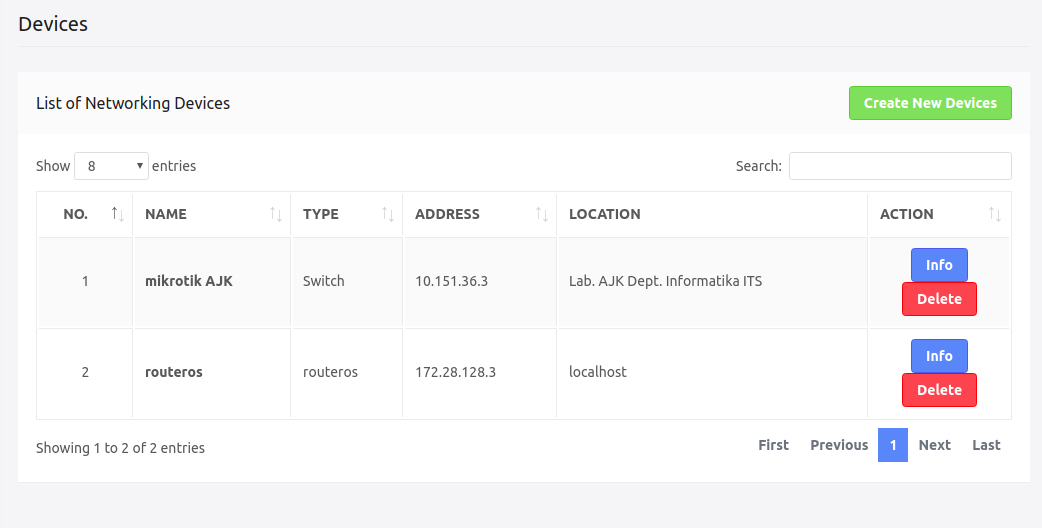
\includegraphics[width=11.2cm]{Images/C-4/antarmukadaftarperangkat.png}
				\caption{Dasbor Daftar Aplikasi}
				\label{antarmuka:daftarperangkat}
			\end{figure}
            
         \subsection{Menampilkan rincian data perangkat jaringan yang terdaftarpada sistem}
         	Halaman ini berfungsi untuk menunjukkan informasi tiap perangkat. Informasi yang disajikan meliputi informasi umum tiap perangkat (nama perangkat, tipe perangkat, alamat perangkat dan lokasi perangkat), daftar pengguna yang berlangganan ke perangkat tersebut, dan daftar OID (informasi keadaan perangkat) yang tersedia pada perangkat tersebut.
         	
         	Pada halaman ini pengguna dapat berlangganan kepada perangkat dengan menekan tombol subscribe pada kolom "\textit{Subscriber}". setelah berhasil berlangganan kepada perangkat, sistem akan menampilkan tombol "\textit{subscribe}" pada kolom OID, dimana tombol tersebut berfungsi untuk memilih informasi apa saja yang ingin didapatkan oleh pengguna. Antarmuka informasi ditunjukkan pada Gambar \ref{antarmuka:rincianperangkat}.
         	\begin{figure}[H]
         		\centering
         		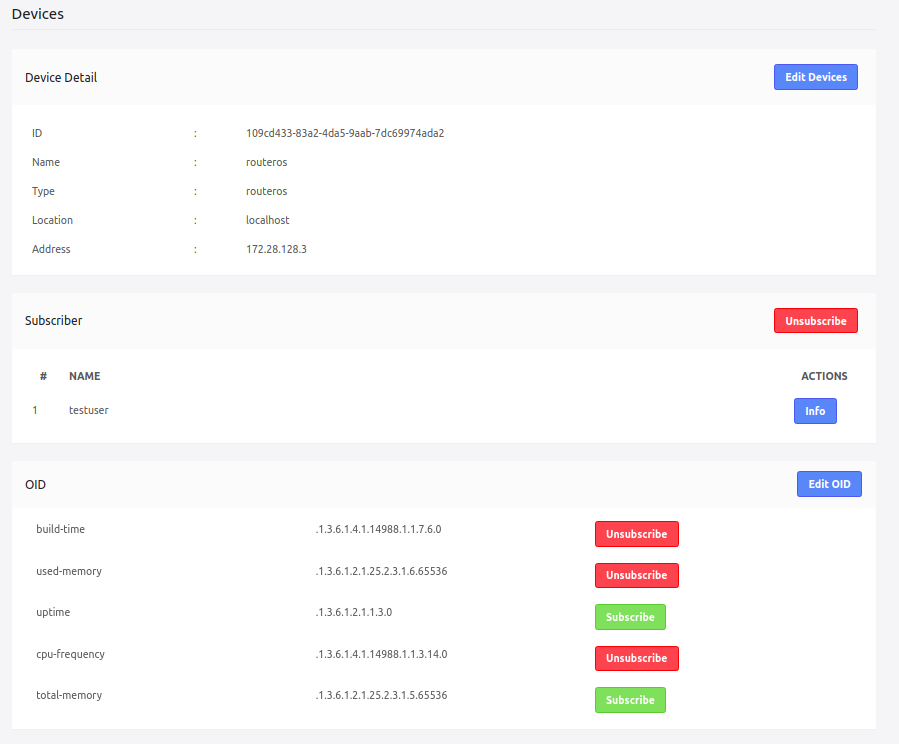
\includegraphics[width=11.2cm]{Images/C-4/antarmukarincianperangkat.png}
         		\caption{Dasbor Informasi Aplikasi}
         		\label{antarmuka:rincianperangkat}
         	\end{figure}
            
         \subsection{Menampilkan data yang ingin dipantau pengguna pada sistem}
         	Pada halaman ini, pengguna dapat memantau atau melihat kondisi dari tiap perangkat yang telah dilanggani oleh tiap pengguna. Informasi yang disajikan pada halaman ini tergantung dari banyaknya informasi pada tiap perangkat yang dilanggani oleh pengguna. pada halaman ini juga, websocket bekerja. jika \textit{client} (\textit{browser}) terkoneksi dengan websocket, maka akan terdapat kotak berwarna hijau pada bagian atas halaman, sedangkan jika \textit{client} tidak terhubung dengan websocket maka kotak tersebut akan berwarna merah. Antarmuka halaman daftar \textit{container} ditunjukkan pada Gambar \ref{antarmuka:pantau}.
            \begin{figure}[H]
				\centering
				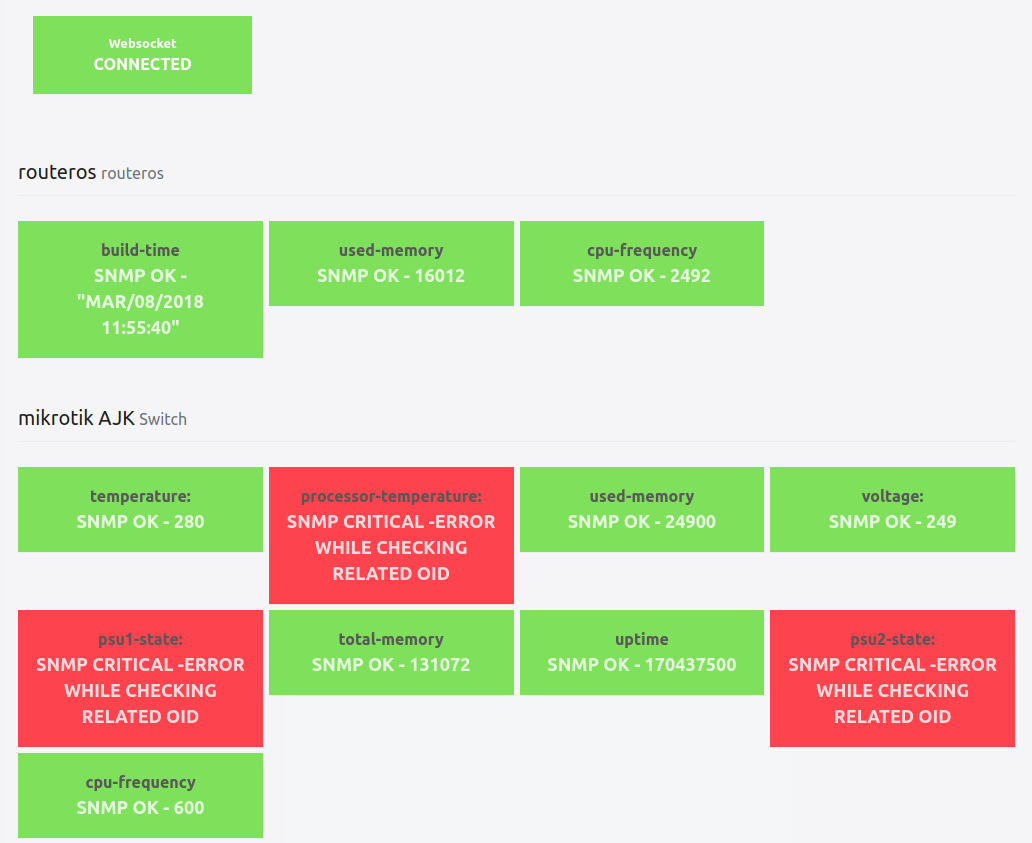
\includegraphics[width=11.2cm]{Images/C-4/antarmukapantau.png}
				\caption{Dasbor Daftar \textit{Container}}
				\label{antarmuka:pantau}
			\end{figure}
	\chapter{PENGUJIAN DAN EVALUASI}

\section{Lingkungan Uji Coba}
	Lingkungan pengujian menggunakan komponen-komponen yang terdiri dari: satu \textit{server publisher}, satu \textit{server publish/subscribe}, satu \textit{server aplikasi}, satu \textit{server API}, satu \textit{server database}, satu agen SNMP dan satu komputer penguji. Semua \textit{server} menggunakan vitual machine yang dipasang pada \textit{Hypervisor} Proxmox. Lalu, untuk komputer penguji menggunakan satu buah laptop sebagai klien yang digunakan untuk menerima data yang dikirim oleh publisher dan melakukan skenario pengetesan pada REST API. Pengujian dilakukan di Laboratoriom Arsitektur dan Jaringan Komputer Jurusan Teknik Informatika ITS. \\
    \indent Spesifikasi untuk setiap komponen yang digunakan ditunjukkan pada Tabel \ref{spesifikasikomponen}.
    \begin{longtable}{|p{0.05\textwidth}|p{0.18\textwidth}|p{0.33\textwidth}|p{0.33\textwidth}|}					\caption{Spesifikasi Komponen} \label{spesifikasikomponen} \\
        \hline
        \textbf{No} & \textbf{Komponen} & \textbf{Perangkat Keras} & \textbf{Perangkat Lunak} \\ \hline
        \endfirsthead
        \caption[]{Spesifikasi Komponen} \\
        \hline
        \textbf{No} & \textbf{Komponen} & \textbf{Perangkat Keras} & \textbf{Perangkat Lunak} \\ \hline
        \endhead
        \endfoot
        \endlastfoot

    	1 & Publisher & 1 core processor, 512 MB RAM, 20GB HDD pada virtualisasi Proxmox & Ubuntu 16.04 LTS, Python2.7, Nagios \\ \hline
        2 & Pub/Sub & 1 core processor, 512 MB RAM, 20GB HDD pada virtualisasi Proxmox & Ubuntu 16.04 LTS, RabbitMQ \\ \hline
        3 & Application & 1 core processor, 512 MB RAM, 20GB HDD pada virtualisasi Proxmox & Ubuntu 16.04 LTS, Node.JS, Python 2.7 \\ \hline
        4 & REST API & 1 core processor, 512 MB RAM, 20GB HDD pada virtualisasi Proxmox & Ubuntu 16.04 LTS, Docker 17.03.0-ce, Python 2.7 \\ \hline
        5 & Database & 1 core processor, 512 MB RAM, 20GB HDD pada virtualisasi Proxmox & Ubuntu 16.04 LTS, MySQL Server \\ \hline
        6 & Agen SNMP & Mikrotik Routerboard Cloud Switch Series & Agen SNMP \\ \hline
        7 & Komputer penguji & Processor Intel i5-3210M, 8 GB RAM & Ubuntu 16.04 LTS, JMeter 4.0 \\ \hline
    \end{longtable}
    
    \indent Untuk akses ke masing-masing komponen, digunakan IP private yang disediakan untuk masing-masing komponen tersebut. Detailnya ditunjukkan pada Tabel \ref{ipdomainserver}.
    			\begin{longtable}{|p{0.05\textwidth}|p{0.33\textwidth}|p{0.44\textwidth}|}					\caption{IP dan Domain Server} \label{ipdomainserver} \\
					\hline
					\textbf{No} & \textbf{Server} & \textbf{IP dan Domain} \\ \hline
					\endfirsthead
					\caption[]{IP dan Domain Server} \\
					\hline
					\textbf{No} & \textbf{Server} & \textbf{IP dan Domain} \\ \hline
					\endhead
					\endfoot
					\endlastfoot
					
                    1 & Publisher & 10.151.36.97 \\ \hline
                    2 & Pub/Sub & 10.151.36.98 \\ \hline
                    3 & Application & 10.151.36.99 \\ \hline
                    4 & REST API & 10.151.36.100 \\ \hline
                    5 & Database & 10.151.36.101 \\ \hline
                    6 & Agen SNMP & 10.151.36.3 \\ \hline
                    7 & Komputer Penguji & 10.151.36.153 \\ \hline
				\end{longtable}
    
\section{Skenario Uji Coba} \label{skenarioujicoba}
	Uji coba akan dilakukan untuk mengetahui keberhasilan sistem yang telah dibangun. Skenario pengujian dibedakan menjadi 2 bagian, yaitu:
    \begin{itemize}
    \item \textbf{Uji Fungsionalitas} \\
    	Pengujian ini didasarkan pada fungsionalitas yang disajikan sistem.
    \item \textbf{Uji Performa} \\
    	Pengujian ini untuk menguji kecepatan respon sistem terhadap sejumlah permintaan ke aplikasi secara bersamaan. Pengujian dilakukan dengan melakukan \textit{benchmark} pada sistem.
    \end{itemize}
    
    \subsection{Skenario Uji Coba Fungsionalitas}
    	Uji fungsionalitas dibagi menjadi 2, yaitu uji fungsionalitas antarmuka aplikasi dan uji fungsionalitas endpoint REST API.
        
        \subsubsection{Uji Fungsionalitas Antarmuka Aplikasi} \label{ujifungsionalitasantarmuka}
        	Pengujuian ini dilakukan untuk memeriksa apakah semua fungsi yang berada pada aplikasi dapat dijalankan dengan benar. Pengujian dilakukan dengan cara mengakses antarmuka yang berhubungan dengan tugas akhir ini lalu menjalankan fitur yang disediakan pada tiap-tiap antarmuka.
        	
        	Rancangan pengujian dan hasil yang diharapkan dapat dilihat pada tabel \ref{ujiaplikasi}.
        	
            \begin{longtable}{|p{0.05\textwidth}|p{0.20\textwidth}|p{0.30\textwidth}|p{0.27\textwidth}|}					\caption{Skenario Uji Fungsionalitas Antarmuka Aplikasi} \label{ujiaplikasi} \\
					\hline
					\textbf{No} & \textbf{Fitur} & \textbf{Uji Coba} & \textbf{Hasil Harapan} \\ \hline
					\endfirsthead
					\caption[]{Skenario Uji Fungsionalitas Antarmuka Aplikasi} \\
					\hline
					\textbf{No} & \textbf{Fitur} & \textbf{Uji Coba} & \textbf{Hasil Harapan} \\ \hline
					\endhead
					\endfoot
					\endlastfoot
					
                    1 & Autentikasi pengguna untuk masuk kedalam sistem. & Pengguna memasukkan username dan password masing-masing milik pengguna pada form yang telah disediakan. & Pengguna dapat masuk ke halaman utama aplikasi setelah menekan tombol "login"\\ \hline
                    2 & Menampilkan seluruh data perangkat. & Pengguna menekan \textit{menu} "DEVICE MANAGEMENT" pada \textit{sidebar}. & Sistem menampilkan seluruh data perangkat yang terdaftar pada sistem. data yang ditampilkan meliputi: nama perangkat, tipe perangkat, alamat perangkat dan lokasi perangkat. serta terdapat tombol informasi untuk melihat data masing-masing perangkat secara rinci dan tombol hapus untuk menghapus data perangkat yang terdaftar pada sistem. \\ \hline
                    3 & Menampilkan rincian data perangkat & Pengguna menekan tombol informasi yang tersedia pada tabel pada halaman menampilkan seluruh data perangkat. & Sistem menampilkan data perangkat terkait secara rinci. data yang ditampilkan meliputi: profil perangkat, pelanggan dari perangkat dan OID (Informasi yang disediakan pada perangkat terkait). \\ \hline
                    4 & Menghapus data perangkat. & Pengguna menekan tombol hapus yang tersedia pada tabel pada halaman menampilkan seluruh data perangkat. & Sistem menghapus data perangkat terkait secara permanen. \\ \hline
					5 & Menyunting data perangkat. & Pengguna menekan tombol ubah data pada halaman rincian data perangkat lalu mengubah data yang tersedia pada form yang berisi data sebelumnya. & Sistem mengubah data yang lama dengan data yang baru dimasukkan oleh pengguna. \\ \hline
                    6 & Berlangganan Data Perangkat. & Pengguna menekan tombol "Subscribe" yang tersedia pada halaman rincian data perangkat. & Sistem menandai bahwa perangkat atau OID (Informasi pada perangkat) yang terkait telat dilanggani. tombol akan berubah menjadi "Unsubscribe"\\ \hline
                    7 & Memantau kondisi perangkat yang telah dilanggani. & Pengguna menekan \textit{menu} "MONITOR" pada \textit{sidebar}. & Sistem menampilkan kondisi dari seluruh perangkat yang telah dilanggani informasinya oleh pengguna. \\ \hline
				\end{longtable}
            
        \subsubsection{Uji Fungsionalitas Endpoint REST API}\label{ujifungsionalitasrestapi}
        	Pengujian ini dilakukan untuk memeriksa apakah seluruh fungsi dan \textit{endpoint} yang berhubungan dengan tugas akhir ini dan tersedia pada sistem dapat bekerja dengan semestinya. Pengujian dilakukan dengan cara mengakses \textit{endpoint} dengan metode tertentu disertai dengan \textit{header} autentikasi JWT . Rancangan pengujian dan hasil yang diharapkan ditunjukkan dengan Tabel \ref{ujirestapi}.
            
            \begin{longtable}{|p{0.05\textwidth}|p{0.20\textwidth}|p{0.30\textwidth}|p{0.27\textwidth}|}					\caption{Skenario Uji Fungsionalitas REST API} \label{ujirestapi} \\
            	\hline
            	\textbf{No} & \textbf{\textit{Endpoint}} & \textbf{Uji Coba} & \textbf{Hasil Harapan} \\ \hline
            	\endfirsthead
            	\caption[]{Skenario Uji Fungsionalitas REST API} \\
            	\hline
            	\textbf{No} & \textbf{\textit{Endpoint}} & \textbf{Uji Coba} & \textbf{Hasil Harapan} \\ \hline
            	\endhead
            	\endfoot
            	\endlastfoot
            	
            	1 & /login. & Mengakses endpoint dengan header autentikasi JWT dan metode POST, disertai dengan body bertipe JSON yang dilengkapi dengan beberapa parameter seperti: username dan password. & REST API mengembalikan respon berupa pesan berhasil dan token JWT jika berhasil, lalu mengembalikan pesan gagal jika gagal. \\ \hline
            	2 & /devices. & Mengakses endpoint dengan header autentikasi JWT dan metode GET. & jika berhasil, REST API mengembalikan respon berupa seluruh data yang tersedia pada sistem dalam bentuk json. tiap datanya meliputi: nama perangkat, tipe perangkat, alamat perangkat dan lokasi perangkat. Jika terjadi kegagalan, REST API akan mengembalikan pesan gagal. \\ \hline
            	3 & /devices/ <string:id> & Mengakses endpoint dengan header autentikasi JWT, metode GET dan menyertakan ID perangkat pada endpoint. & jika berhasil, REST API mengembalikan respon berupa seluruh data yang tersedia pada sistem dalam bentuk json. tiap datanya meliputi: nama perangkat, tipe perangkat, alamat perangkat, lokasi perangkat, subscriber perangkat dan OID (informasi yang tersedia pada perangkat). Jika terjadi kegagalan, REST API akan mengembalikan pesan gagal. \\ \hline
            	4 & /devices /create. & Mengakses endpoint dengan header autentikasi JWT dan metode POST, disertai dengan body bertipe JSON yang dilengkapi dengan beberapa parameter seperti: \textit{name}, \textit{type}, \textit{address} dan \textit{location} & jika berhasil, REST API mengembalikan respon berupa pesan berhasil. Jika gagal, maka REST API akan mengambalikan pesan gagal. \\ \hline
            	5 & /devices /edit /<string:id> & Mengakses endpoint dengan header autentikasi JWT, metode POST, menyertakan ID perangkat pada endpoint dan disertai dengan body bertipe JSON yang dilengkapi dengan beberapa parameter seperti: \textit{name}, \textit{type}, \textit{address} dan \textit{location}. & jika berhasil, REST API mengembalikan respon berupa pesan berhasil. Jika gagal, maka REST API akan mengambalikan pesan gagal. \\ \hline
            	6 & /devices /delete & Mengakses endpoint dengan header autentikasi JWT dan metode DELETE, disertai dengan body bertipe JSON yang dilengkapi dengan parameter ID perangkat. & jika berhasil, REST API mengembalikan respon berupa pesan berhasil. Jika gagal, maka REST API akan mengambalikan pesan gagal. \\ \hline
            	7 & /oid /create & Mengakses endpoint dengan header autentikasi JWT dan metode POST, disertai dengan body bertipe JSON yang dilengkapi dengan beberapa parameter seperti: oidname, oid dan devices\_id & jika berhasil, REST API mengembalikan respon berupa pesan berhasil. Jika gagal, maka REST API akan mengambalikan pesan gagal. \\ \hline
            	8 & /oid /edit & Mengakses endpoint dengan header autentikasi JWT dan metode POST, disertai dengan body bertipe JSON yang dilengkapi dengan beberapa parameter seperti: oidname, oid dan devices\_id & jika berhasil, REST API mengembalikan respon berupa pesan berhasil. Jika gagal, maka REST API akan mengambalikan pesan gagal. \\ \hline
            	9 & /oid /delete & Mengakses endpoint dengan header autentikasi JWT dan metode POST, disertai dengan body bertipe JSON yang dilengkapi dengan parameter parameter ID perangkat. & jika berhasil, REST API mengembalikan respon berupa pesan berhasil. Jika gagal, maka REST API akan mengambalikan pesan gagal. \\ \hline
            	10 & /subscribe /devices & Mengakses endpoint dengan header autentikasi JWT dan metode POST, disertai dengan body bertipe JSON yang dilengkapi dengan beberapa parameter seperti: device\_id dan users\_id. & jika berhasil, REST API mengembalikan respon berupa pesan berhasil. Jika gagal, maka REST API akan mengambalikan pesan gagal. \\ \hline
            	11 & /unsubscribe /devices & Mengakses endpoint dengan header autentikasi JWT dan metode POST, disertai dengan body bertipe JSON yang dilengkapi dengan beberapa parameter seperti: device\_id dan users\_id. & jika berhasil, REST API mengembalikan respon berupa pesan berhasil. Jika gagal, maka REST API akan mengambalikan pesan gagal. \\ \hline
            	12 & /subscribe /oid & Mengakses endpoint dengan header autentikasi JWT dan metode POST, disertai dengan body bertipe JSON yang dilengkapi dengan beberapa parameter seperti: oid\_id dan users\_id. & jika berhasil, REST API mengembalikan respon berupa pesan berhasil. Jika gagal, maka REST API akan mengambalikan pesan gagal. \\ \hline
            	13 & /unsubscribe /oid & Mengakses endpoint dengan header autentikasi JWT dan metode POST, disertai dengan body bertipe JSON yang dilengkapi dengan beberapa parameter seperti: oid\_id dan users\_id. & jika berhasil, REST API mengembalikan respon berupa pesan berhasil. Jika gagal, maka REST API akan mengambalikan pesan gagal. \\ \hline
            \end{longtable}
            
        
    \subsection{Skenario Uji Coba Performa}
    	Uji performa dilakukan dengan dua langkah, yaitu uji performa REST api dan uji performa publish/subscribe. Arsitektur sistem yang dirancang untuk pengujian dapat dilihat pada gambar \ref{arsitekturpengujian}.
    	
    	Uji coba REST API dilakukan dengan menggunakan satu buah laptop untuk melakukan akses secara bersamaan ke REST API menggunakan aplikasi JMeter. Laptop akan mencoba mengaskses REST API yang sudah berjalan pada suatu server, dengan alamat IP 10.151.36.100.
    	
    	Uji performa selanjutnya yaitu uji performa publish/subscribe dilakukan dengan cara menghitung waktu pengiriman. pengiriman dilakukan dari publisher yang berada pada server dengan alamat IP 10.151.36.97 menuju consumer yang berada pada alamat IP 10.151.36.99.
    	
    	\begin{figure}[H]
    		\centering
    		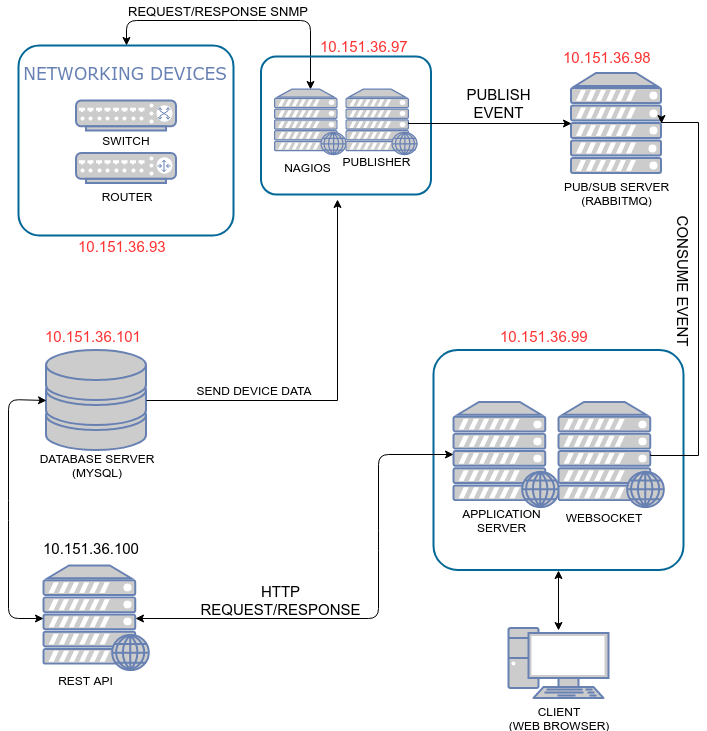
\includegraphics[width=9cm]{Images/C-5/arsitesting.png}
    		\caption{Arsitektur Sistem yang Digunakan Untuk Pengujian}
    		\label{arsitekturpengujian}
    	\end{figure}
        
    	\subsubsection{Uji Performa Kecepatan REST API Menangani \textit{Request}}
        	Pengujian dilakukan dengan mengukur jumlah waktu yang diperlukan oleh REST API untuk menyelesaikan \textit{request} yang dilakukan oleh komputer penguji. Waktu yang diukur adalah perbedaan jarak antara \textit{request} pertama dan terakhir dilakukan oleh klien yang mendapatkan balasan dari \textit{server}.
        	
        	Percobaan dilakukan dengan membuat thread untuk setiap akses ke REST API. Pengujian akan berlangsung bertahap mulai dari 300, 600, 900, 1200 dan 1500 thread dengan pengulangan 5 kali untuk setiap \textit{event}. Dari hasil pengujian akan didapatkan waktu respon terhadap permintaan. Waktu tersebut digunakan untuk membuat grafik kesimpulan.
        \subsubsection{Uji Performa Kecepatan Pengiriman Data Dari Publisher Menuju Consumer}
        	Pengujian dilakukan dengan menghitung waktu yang diperlukan publisher untuk mengirimkan data hingga sampai kepada consumer melalui pub/sub server. Pengujian dilakukan dengan cara mengurangi waktu (timestamp) yang dideklarasikan saat publisher mengirimkan data dengan waktu (timestamp) saat pesan sampai di consumer dan siap untuk dikirimkan kepada client melalu websocket.
    
\section{Hasil Uji Coba dan Evaluasi}
	Berikut dijelaskan hasil uji coba dan evaluasi berdasarkan skenario yang telah dijelaskan pada subbab \ref{skenarioujicoba}.
    
	\subsection{Uji Fungsionalitas}
    	Berikut dijelaskan hasil pengujian fungsionalitas pada sistem yang dibangun.
        
        \subsubsection{Uji Fungsionalitas Antarmuka Aplikasi}
    	Pengujian dilakukan sesuai dengan skenario yang dijelaskan pada subbab \ref{ujifungsionalitasantarmuka} dan pada Tabel \ref{ujiaplikasi}. Hasil pengujian seperti tertera pada Tabel \ref{hasilujicobaaplikasi}.
        
        \begin{longtable}{|p{0.05\textwidth}|p{0.55\textwidth}|p{0.22\textwidth}|}					\caption{Hasil Uji Coba Mengelola Aplikasi Berbasis Docker} \label{hasilujicobaaplikasi} \\
					\hline
					\textbf{No} & \textbf{Uji Coba} & \textbf{Hasil} \\ \hline
					\endfirsthead
					\caption[]{Hasil Uji Coba Mengelola Aplikasi Berbasis Docker} \\
					\hline
					\textbf{No} & \textbf{Uji Coba} & \textbf{Hasil} \\ \hline
					\endhead
					\endfoot
					\endlastfoot
					
                    1 & Pengguna memasukkan username dan password masing-masing milik pengguna pada form yang telah disediakan. & Sukses \\ \hline
                    2 & Pengguna menekan \textit{menu} "DEVICE MANAGEMENT" pada \textit{sidebar}. & Sukses \\ \hline
                    3 & Pengguna menekan tombol informasi yang tersedia pada tabel pada halaman menampilkan seluruh data perangkat. & Sukses \\ \hline
                    4 & Pengguna menekan tombol hapus yang tersedia pada tabel pada halaman menampilkan seluruh data perangkat. & Sukses \\ \hline
					5 & Pengguna menekan tombol ubah data pada halaman rincian data perangkat lalu mengubah data yang tersedia pada form yang berisi data sebelumnya. & Sukses \\ \hline
                    6 & Pengguna menekan tombol "Subscribe" yang tersedia pada halaman rincian data perangkat. & Sukses \\ \hline
					7 & Pengguna menekan \textit{menu} "MONITOR" pada \textit{sidebar}. & Sukses \\ \hline
				\end{longtable}
    		Sesuai dengan skenario uji coba  yang diberikan pada Tabel \ref{ujiaplikasi}, hasil uji coba menunjukkan semua skenario berhasil ditangani.
        
    	\subsubsection{Uji Fungsionalitas Endpoint REST API}
        	Pengujian dilakukan sesuai dengan skenario yang dijelaskan pada subbab \ref{ujifungsionalitasrestapi} dan pada Tabel \ref{ujirestapi}. Hasil pengujian seperti tertera pada Tabel \ref{hasilujirestapi}.
        	
        		\begin{longtable}{|p{0.05\textwidth}|p{0.20\textwidth}|p{0.30\textwidth}|p{0.27\textwidth}|}					\caption{Skenario Uji Fungsionalitas REST API} \label{hasilujirestapi} \\
        			\hline
        			\textbf{No} & \textbf{\textit{Endpoint}} & \textbf{Uji Coba} & \textbf{Hasil Harapan} \\ \hline
        			\endfirsthead
        			\caption[]{Skenario Uji Fungsionalitas REST API} \\
        			\hline
        			\textbf{No} & \textbf{\textit{Endpoint}} & \textbf{Uji Coba} & \textbf{Hasil} \\ \hline
        			\endhead
        			\endfoot
        			\endlastfoot
        			
        			1 & /login. & Mengakses endpoint dengan header autentikasi JWT dan metode POST, disertai dengan body bertipe JSON yang dilengkapi dengan beberapa parameter seperti: username dan password. & OK - REST API mengembalikan respon berupa pesan berhasil \\ \hline
        			2 & /devices. & Mengakses endpoint dengan header autentikasi JWT dan metode GET. & OK - REST API mengembalikan respon berupa seluruh data yang tersedia pada sistem dalam bentuk json. tiap datanya meliputi: nama perangkat, tipe perangkat, alamat perangkat dan lokasi perangkat. \\ \hline
        			3 & /devices/ <string:id> & Mengakses endpoint dengan header autentikasi JWT, metode GET dan menyertakan ID perangkat pada endpoint. & OK - REST API mengembalikan respon berupa seluruh data yang tersedia pada sistem dalam bentuk json. tiap datanya meliputi: nama perangkat, tipe perangkat, alamat perangkat, lokasi perangkat, subscriber perangkat dan OID (informasi yang tersedia pada perangkat). \\ \hline
        			4 & /devices /create. & Mengakses endpoint dengan header autentikasi JWT dan metode POST, disertai dengan body bertipe JSON yang dilengkapi dengan beberapa parameter seperti: \textit{name}, \textit{type}, \textit{address} dan \textit{location} & OK - REST API mengembalikan respon berupa pesan berhasil. \\ \hline
        			5 & /devices /edit /<string:id> & Mengakses endpoint dengan header autentikasi JWT, metode POST, menyertakan ID perangkat pada endpoint dan disertai dengan body bertipe JSON yang dilengkapi dengan beberapa parameter seperti: \textit{name}, \textit{type}, \textit{address} dan \textit{location}. & OK - REST API mengembalikan respon berupa pesan berhasil. \\ \hline
        			6 & /devices /delete & Mengakses endpoint dengan header autentikasi JWT dan metode DELETE, disertai dengan body bertipe JSON yang dilengkapi dengan parameter ID perangkat. & OK - REST API mengembalikan respon berupa pesan berhasil. \\ \hline
        			7 & /oid /create & Mengakses endpoint dengan header autentikasi JWT dan metode POST, disertai dengan body bertipe JSON yang dilengkapi dengan beberapa parameter seperti: oidname, oid dan devices\_id & OK - REST API mengembalikan respon berupa pesan berhasil. \\ \hline
        			8 & /oid /edit & Mengakses endpoint dengan header autentikasi JWT dan metode POST, disertai dengan body bertipe JSON yang dilengkapi dengan beberapa parameter seperti: oidname, oid dan devices\_id & OK - REST API mengembalikan respon berupa pesan berhasil. \\ \hline
        			9 & /oid /delete & Mengakses endpoint dengan header autentikasi JWT dan metode POST, disertai dengan body bertipe JSON yang dilengkapi dengan parameter parameter ID perangkat. & OK - REST API mengembalikan respon berupa pesan berhasil. \\ \hline
        			10 & /subscribe /devices & Mengakses endpoint dengan header autentikasi JWT dan metode POST, disertai dengan body bertipe JSON yang dilengkapi dengan beberapa parameter seperti: device\_id dan users\_id. & OK - REST API mengembalikan respon berupa pesan berhasil. \\ \hline
        			11 & /unsubscribe /devices & Mengakses endpoint dengan header autentikasi JWT dan metode POST, disertai dengan body bertipe JSON yang dilengkapi dengan beberapa parameter seperti: device\_id dan users\_id. & OK - REST API mengembalikan respon berupa pesan berhasil. \\ \hline
        			12 & /subscribe /oid & Mengakses endpoint dengan header autentikasi JWT dan metode POST, disertai dengan body bertipe JSON yang dilengkapi dengan beberapa parameter seperti: oid\_id dan users\_id. & OK - REST API mengembalikan respon berupa pesan berhasil. \\ \hline
        			13 & /unsubscribe /oid & Mengakses endpoint dengan header autentikasi JWT dan metode POST, disertai dengan body bertipe JSON yang dilengkapi dengan beberapa parameter seperti: oid\_id dan users\_id. & OK - REST API mengembalikan respon berupa pesan berhasil. \\ \hline
        		\end{longtable}
    \pagebreak
    \subsection{Hasil Uji Performa}
    	Seperti yang sudah dijelaskan pada subbab \ref{skenarioujicoba} pengujian performa dilakukan dengan menghitung respon dari sistem terhadap sejumlah permintaan (\textit{request}) secara bersamaan.
        \begin{longtable}{|p{0.33\textwidth}|p{0.35\textwidth}|}
        \caption{Jumlah \textit{Request} ke Aplikasi} \label{trequest} \\
            \hline
            \textbf{\textit{Concurrent Users}} & \textbf{Jumlah \textit{Request}} \\ \hline
            \endfirsthead
            \caption[]{Jumlah \textit{Request} ke Aplikasi} \\
            \hline
            \textbf{\textit{Concurrent Users}} & \textbf{Jumlah \textit{Request}} \\ \hline
            \endhead
            \endfoot
            \endlastfoot
            
            800 & $\pm$ 16.925 \\ \hline
            1.600 & $\pm$ 26.650 \\ \hline
            2.400 & $\pm$ 34.943 \\ \hline
            3.200 & $\pm$ 50.092 \\ \hline
            4.000 & $\pm$ 57.750 \\ \hline
					
		\end{longtable}
        
        Pada Tabel \ref{tjumlahcontainer} dapat dilihat jumlah \textit{container} yang terbentuk selama proses \textit{request} dari \textit{user} yang dilakukan selama enam kali. Nilai yang ditampilkan berupa nilai rata-rata selama percobaan dibulatkan ke atas. Sistem dapat menyediakan \textit{container} sesuai dengan jumlah \textit{request} yang diberikan, semakin banyak \textit{request} yang dilakukan, maka \textit{container} yang disediakan akan semakin banyak. Nilai \textit{container} tersebut didapatkan dari perhitungan \textit{proactive model}. Selain melihat jumlah \textit{request}, penentuan \textit{container} yang dibentuk juga dari jumlah sumber daya yang digunakan \textit{container} berdasarkan perhitungan menggunakan \textit{reactive model}. Pada Gambar \ref{gjumlahcontainer} dapat dilihat grafik dari jumlah \textit{container} yang terbentuk berdasarkan jumlah \textit{request} yang dilakukan.
        
        \begin{longtable}{|p{0.25\textwidth}|p{0.20\textwidth}|p{0.20\textwidth}|}
        \caption{Jumlah \textit{Container}} \label{tjumlahcontainer} \\
            \hline
            \textbf{\textit{Concurrent Users}} & \textbf{Maksimal \textit{Container}} &  \textbf{Rata-rata \textit{Container}} \\ \hline
            \endfirsthead
            \caption[]{Jumlah \textit{Container}} \\
            \hline
            \textbf{\textit{Concurrent Users}} & \textbf{Maksimal \textit{Container}} &  \textbf{Rata-rata \textit{Container}} \\ \hline
            \endhead
            \endfoot
            \endlastfoot
            
            800 & 6 & 2 \\ \hline
            1.600 & 8 & 3 \\ \hline
            2.400 & 14 & 6 \\ \hline
            3.200 & 18 & 7 \\ \hline
            4.000 & 30 & 11 \\ \hline
					
		\end{longtable}
        
        \begin{figure}[H]
				\centering
				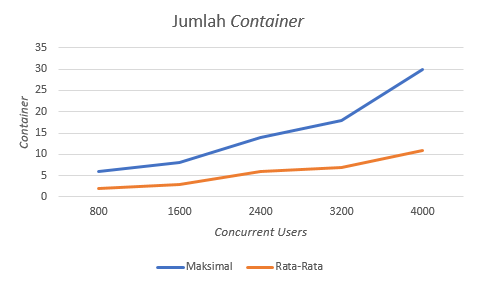
\includegraphics[width=8.7cm,height=4.7cm]{Images/C-5/jumlahcontainer.png}
				\caption{Grafik Jumlah \textit{Container}}
				\label{gjumlahcontainer}
			\end{figure}
        
    	\subsubsection{Kecepatan Menangani \textit{Request}}
        	Dari hasil uji coba kecepatan menangani \textit{request}, dapat dilihat pada Table \ref{kecepatanrequest} dalam satuan detik bahwa semakin banyak \textit{concurrent users}, semakin lama pula waktu yang diperlukan untuk menyeselaikannya. Request paling cepat ditangani dengan menggunakan prediksi ARIMA(4,1,0) dan paling lambat menggunakan ARIMA(1,1,0). Hal tersebut terjadi karena kurang bagusnya hasil prediksi yang dihasilkan oleh ARIMA(1,1,0) yang mana kadang hasil prediksinya terlalu rendah atau terlalu tinggi.
            Dari hasil percobaan tersebut, dapat dilihat bahwa hampir semua \textit{request} dapat ditangani di bawah satu menit. Lalu grafik hasil uji coba perhitungan kecepatan menangani \textit{request} ditunjukkan pada Gambar \ref{grunningtime}.
            \begin{longtable}{|p{0.22\textwidth}|p{0.10\textwidth}|p{0.10\textwidth}|p{0.10\textwidth}|p{0.10\textwidth}|p{0.10\textwidth}|}
        \caption{Kecepatan Menangani \textit{Request}} \label{kecepatanrequest} \\
            \hline
            & \textbf{800} & \textbf{1600} & \textbf{2400} & \textbf{3200} & \textbf{4000} \\ \hline
            \endfirsthead
            \caption[]{Kecepatan Menangani \textit{Request}} \\
            \hline
            & \textbf{800} & \textbf{1600} & \textbf{2400} & \textbf{3200} & \textbf{4000} \\ \hline
            \endhead
            \endfoot
            \endlastfoot
			
          	ARIMA(1,1,0) & 34.167 & 43.286 & 48.143 & 63.857 & 62.286 \\ \hline
            ARIMA(2,1,0) & 27.429 & 38.571 & 44.143 & 42.143 & 57.857 \\ \hline
            ARIMA(3,1,0) & 32.429 & 36.000 & 38.429 & 41.571 & 43.857 \\ \hline
            ARIMA(4,1,0) & 24.857 & 31.571 & 34.429 & 42.143 & 52.714 \\ \hline
		\end{longtable}
         
        	\begin{figure}[H]
				\centering
				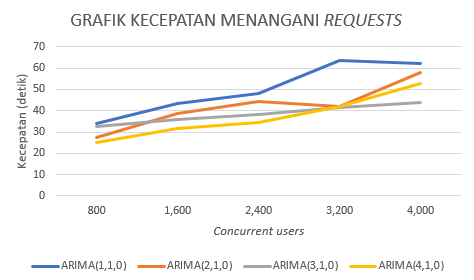
\includegraphics[width=8.7cm,height=4.7cm]{Images/C-5/runningtime.png}
				\caption{Grafik Kecepatan Menangani \textit{Request}}
				\label{grunningtime}
			\end{figure}
            
        \subsubsection{Penggunaan CPU}
        	Dari hasil uji coba penggunaan CPU pada \textit{server master host}, penggunaan CPU berada di bawah 15\%. Penggunaan CPU yang diukur adalah penggunaan CPU yang dilakukan oleh \textit{container} dari aplikasi, tidak termasuk sistem. Jumlah \textit{core} yang dimiliki oleh \textit{processor} di \textit{server master host} adalah 8 buah, yang artinya kurang lebih hanya satu core yang digunakan untuk menangani semua \textit{request}. Hasil pengukuran penggunaan CPU dapat dilihat pada Tabel \ref{penggunaancpu}
            
            \begin{longtable}{|p{0.22\textwidth}|p{0.10\textwidth}|p{0.10\textwidth}|p{0.10\textwidth}|p{0.10\textwidth}|p{0.10\textwidth}|}
        \caption{Penggunaan CPU} \label{penggunaancpu} \\
            \hline
            & \textbf{800} & \textbf{1600} & \textbf{2400} & \textbf{3200} & \textbf{4000} \\ \hline
            \endfirsthead
            \caption[]{Penggunaan CPU} \\
            \hline
            & \textbf{800} & \textbf{1600} & \textbf{2400} & \textbf{3200} & \textbf{4000} \\ \hline
            \endhead
            \endfoot
            \endlastfoot
			
            ARIMA(1,1,0) & 7.1\% & 7.8\% & 9.1\% & 10.5\% & 10.7\% \\ \hline
            ARIMA(2,1,0) & 8.5\% & 9.2\% & 10.1\% & 11.3\% & 10.7\% \\ \hline
            ARIMA(3,1,0) & 8.8\% & 10.2\% & 11.6\% & 12.1\% & 10.3\% \\ \hline
            ARIMA(4,1,0) & 8.0\% & 8.3\% & 10.1\% & 12.9\% & 10.5\% \\ \hline

		\end{longtable}
            
            Dari hasil uji coba, penggunaan prediksi yang berbeda tidak terlalu berpengaruh terhadap penggunaan CPU. Lalu, penggunaan CPU tergolong rendah, yaitu hanya sebesar $\pm 10 \%$ untuk menangani semua \textit{request} yang diberikan. Hasil uji coba performa penggunaan CPU ditunjukkan oleh dalam grafik pada Gambar \ref{gcpuusage}.
            
        	\begin{figure}[H]
				\centering
				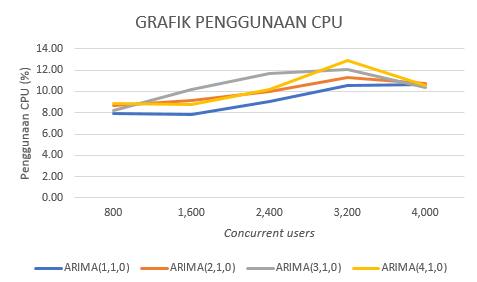
\includegraphics[width=8.7cm,height=4.7cm]{Images/C-5/cpuusage.png}
				\caption{Grafik Penggunaan CPU}
				\label{gcpuusage}
			\end{figure}
            
        \subsubsection{Penggunaan \textit{Memory}}            
            Dari hasil uji coba penggunaan \textit{memory}, semakin banyak \textit{request} yang diterima, semakin banyak \textit{memory} yang diperlukan. Perhitungan penggunaan \textit{memory} adalah rata-rata penggunaan dari masing-masing \textit{container} sebuah aplikasi. Untuk masing-masing \textit{container}, dibatasi penggunaan maksimal \textit{memory} adalah 512 MB. Dari hasil uji coba ini, dapat dilihat pada Tabel \ref{penggunaanmemory} bahwa penggunaan terbesar hanya sebesar 158.71 MB. Artinya jumlah tersebut hanya menggunakan sepertiga dari keseluruhan \textit{memory} yang bisa digunakan.
            \begin{longtable}{|p{0.22\textwidth}|p{0.10\textwidth}|p{0.10\textwidth}|p{0.10\textwidth}|p{0.10\textwidth}|p{0.10\textwidth}|}
        \caption{Penggunaan \textit{Memory}} \label{penggunaanmemory} \\
            \hline
            & \textbf{800} & \textbf{1600} & \textbf{2400} & \textbf{3200} & \textbf{4000} \\ \hline
            \endfirsthead
            \caption[]{Penggunaan \textit{Memory}} \\
            \hline
            & \textbf{800} & \textbf{1600} & \textbf{2400} & \textbf{3200} & \textbf{4000} \\ \hline
            \endhead
            \endfoot
            \endlastfoot
			
           	ARIMA(1,1,0) & 67.91 & 88.97 & 130.79 & 120.14 & 157.73 \\ \hline
            ARIMA(2,1,0) & 65.89 & 97.98 & 123.47 & 156.64 & 158.33 \\ \hline
            ARIMA(3,1,0) & 72.20 & 99.72 & 125.56 & 144.42 & 152.14 \\ \hline
            ARIMA(4,1,0) & 69.60 & 77.34 & 117.39 & 149.76 & 158.71 \\ \hline

		\end{longtable}
            
            Hasil uji coba performa penggunaan \textit{memory} dalam grafik ditunjukkan pada Gambar \ref{gmemoryusage}.
            
        	\begin{figure}[H]
				\centering
				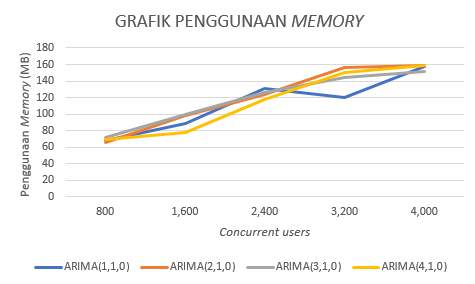
\includegraphics[width=8.7cm,height=4.7cm]{Images/C-5/memoryusage.png}
				\caption{Grafik Penggunaan Memory}
				\label{gmemoryusage}
			\end{figure}
            
        \subsubsection{Keberhasilan \textit{Request}}
        	Pada uji coba ini, dilakukan perhitungan seberapa besar jumlah \textit{request} yang gagal dilakukan. Untuk jumlah \textit{concurrent user} pada tingkat 800 dan 1600, dapat dilihat pada Table \ref{keberhasilanrequest} \textit{error} yang terjadi hampir sama. Prediksi menggunakan ARIMA(4,1,0) berhasil unggul karena menggunakan parameter yang lebih banyak. Namun hal tersebut tidak berlaku untuk ARIMA(3,1,0) karena walaupun parameternya lebih banyak dari ARIMA(2,1,0), tapi hasil prediksinya bisa meleset saat terjadi kondisi dimana koefisien negatif atau koefisien ke dua dikalikan dengan sebuah parameter bukan nol, dan koefisien lain dikalikan dengan parameter nol, maka hasil prediksinya akan negatif, yang mana seharusnya tidak mungkin ada \textit{request} negatif.
            \begin{longtable}{|p{0.22\textwidth}|p{0.10\textwidth}|p{0.10\textwidth}|p{0.10\textwidth}|p{0.10\textwidth}|p{0.10\textwidth}|}
        \caption{\textit{Error Ratio Request}} \label{keberhasilanrequest} \\
            \hline
            & \textbf{800} & \textbf{1600} & \textbf{2400} & \textbf{3200} & \textbf{4000} \\ \hline
            \endfirsthead
            \caption[]{\textit{Error Ratio Request}} \\
            \hline
            & \textbf{800} & \textbf{1600} & \textbf{2400} & \textbf{3200} & \textbf{4000} \\ \hline
            \endhead
            \endfoot
            \endlastfoot
			
            ARIMA(1,1,0) & 5.72\% & 8.96\% & 12.85\% & 12.54\% & 13.38\% \\ \hline
            ARIMA(2,1,0) & 4.31\% & 9.35\% & 10.68\% & 8.11\% & 9.04\% \\ \hline
            ARIMA(3,1,0) & 4.84\% & 10.02\% & 13.22\% & 8.63\% & 12.24\% \\ \hline
            ARIMA(4,1,0) & 4.62\% & 8.41\% & 9.39\% & 7.52\% & 9.21\% \\ \hline
		\end{longtable}
            
    		\begin{figure}[H]
				\centering
				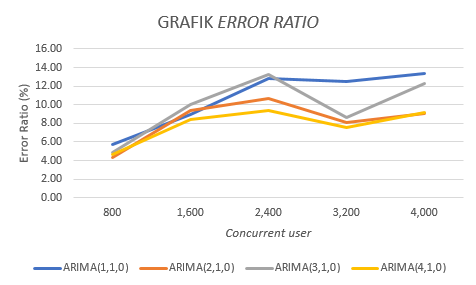
\includegraphics[width=8.7cm,height=4.4cm]{Images/C-5/errorratio.png}
				\caption{Grafik Error Ratio}
				\label{gerrorratio}
			\end{figure}
            Dari uji coba itu, 90\% lebih \textit{request} berhasil ditangani. Hasil uji coba jumlah \textit{request} yang gagal ditunjukkan dengan grafik pada Gambar \ref{gerrorratio}.
	\chapter{PENUTUP}
    Bab ini membahas kesimpulan yang dapat diambil dari tujuan pembuatan sistem dan hubungannya dengan hasil uji coba dan evaluasi yang telah dilakukan. Selain itu, terdapat beberapa saran yang bisa dijadikan acuan untuk melakukan pengembangan dan penelitian lebih lanjut.
        
	\section{Kesimpulan}
        Dari proses perencangan, implementasi dan pengujian terhadap sistem, dapat diambil beberapa kesimpulan berikut:
		\begin{enumerate}
            \item Sistem dapat menjalankan dan menyajikan satu atau lebih aplikasi web berbasis \textit{docker} kepada \textit{end-user} melalui domain yang disediakan.
            \item Sistem dapat menyesuaikan sumber daya secara otomatis berdasarkan jumlah \textit{request} dengan menggunakan \textit{proactive model} dan penggunaan sumber daya, yaitu CPU dan \textit{memory}, pada \textit{container} dengan menggunakan \textit{reactive model}.
            \item Penggunaan \textit{load balancer} cocok digunakan dengan aplikasi yang berjalan di atas \textit{docker} \textit{container}. Hal tersebut karena semua \textit{request} ke aplikasi akan melalui \textit{load balancer}. Jika terjadi penambahan dan pengurangan sumber daya, penyesuaian dengan cepat dilakukan dan hanya perlu merubah sedikit konfigurasi pada \textit{load balancer} dan pengguna tidak perlu tahu apa yang terjadi di dalam sistem.
            \item Prediksi jumlah \textit{request} menggunakan ARIMA sudah bisa menangani skenario uji coba. Perbedaan \textit{order} ARIMA yang digunakan mempengaruhi akurasi dalam menentukan \textit{request} yang akan terjadi ke depannya. Dalam pengujian ini, ARIMA(4,1,0) memiliki hasil pengujian paling bagus dengan jumlah rata-rata \textit{error request} yang paling rendah, yaitu sebesar 7.83\%. Lalu untuk kecepatan menerima \textit{request}, ARIMA(2,1,0) dan ARIMA(4,1,0) memiliki konsistensi yang berbanding lurus dengan jumlah \textit{request}.
            \item Penggunaan sumber daya CPU dan \textit{memory} tidak dipengaruhi oleh penggunaan ARIMA yang berbeda. Penggunaan sumber daya tersebut bergantung kepada jumlah \textit{request}, semakin banyak \textit{request} yang diberikan, penggunaan CPU dan \textit{memory} akan semakin tinggi. Penggunaan CPU paling tinggi yaitu sebesar 12.9\% dan penggunaan \textit{memory} paling tinggi sebesar 158.71 MB. Dengan penggunaan tersebut, masih tersisa lebih dari setengah sumber daya yang bisa digunakan.
            \item Sebuah \textit{container} dari sebuah aplikasi dapat dibentuk dalam waktu $\pm$ 1 detik sehingga penambahan sumber daya bisa dilakukan dengan cepat dan proses untuk memperbarui konfigurasi dari HAProxy memerlukan waktu $\pm$ 5 detik. Selama proses tersebut, akses pengguna akan tertunda, namun tidak menunjukkan terjadinya \textit{down}.
		\end{enumerate}
        
	\section{Saran}
		Berikut beberapa saran yang diberikan untuk pengembangan lebih lanjut:
		\begin{enumerate}
			\item Mengamankan komunikasi antar \textit{server} karena saat ini \textit{endpoint server} bisa diakses oleh siapapun. Hal tersebut bisa dilakukan dengan mengimplentasikan \textit{private} IP dan menggunakan token untuk komunikasinya.
            \item Pemodelan menggunakan ARIMA cukup baik, namun perlu dicoba untuk melakukan pembuatan model dengan \textit{dataset} yang lebih baru. Selain itu, bisa mencoba alternatif pemodelan \textit{time series} yang lain, seperti ARCH (Autoregressive Conditional Heteroskedasticity).
		\end{enumerate}

	\bibliography{Zotero}
	\bibliographystyle{IEEEtranID.bst}
    
    \renewcommand\chaptername{LAMPIRAN}
	\appendix
    \chapter{INSTALASI PERANGKAT LUNAK}

\section*{Instalasi Lingkungan Docker}
	Proses pemasangan Docker dpat dilakukan sesuai tahap berikut:
    \begin{itemize}
    \item Menambahkan repository Docker\\
    	Langkah ini dilakukan untuk menambahkan \textit{repository} Docker ke dalam paket \texttt{apt} agar dapat di unduh oleh Ubuntu. Untuk melakukannya, jalankan perintah berikut:
		\begin{tabbing}
          \texttt{sudo apt-get -y install \char`\\} \\
          \hspace{5 mm} \texttt{apt-transport-https \char`\\} \\
          \hspace{5 mm} \texttt{ca-certificates \char`\\} \\
          \hspace{5 mm} \texttt{curl} \\
          \\
          \texttt{curl -fsSL https://download.docker.com/linux/} \\
          \hspace{7 mm} \texttt{ubuntu/gpg | sudo apt-key add -} \\
          \\
          \texttt{sudo add-apt-repository \char`\\} \\
          \hspace{7 mm} \texttt{"deb [arch=amd64] https://download.docker.com/} \\
          \hspace{9 mm} \texttt{linux/ubuntu \char`\\} \\
          \hspace{7 mm} \texttt{\$ (lsb\_release -cs) \char`\\} \\
          \hspace{7 mm} \texttt{stable"} \\
          \\
          \texttt{sudo apt-get update} \\
        \end{tabbing}
        
    \item Mengunduh Docker \\
    	Docker dikembangkan dalam dua versi, yaitu CE (\textit{Community Edition}) dan EE (\textit{Enterprise Edition}). Dalam pengembangan sistem ini, digunakan Docker CE karena merupakan versi Docker yang gratis. Untuk mengunduh Docker CE, jalankan perintah \texttt{sudo apt-get -y install docker-ce}.
    
    \item Mencoba menjalankan Docker \\
    	Untuk melakukan tes apakah Docker sudah terpasang dengan benar, gunakan perintah \texttt{sudo docker run hello-world}.
    \end{itemize}

\section*{Instalasi Docker Registry} \label{install:dockerRegistry}
	Docker Registry dikembangkan menggunakan Docker Compose. Dengan menggunakan Docker Compose, proses pemasangan Docker Registry menjadi lebih mudah dan fleksibel untuk dikembangkan ditempat lain. Docker Registry akan dijalankan pada satu \textit{container} dan Nginx juga akan dijalankan di satu \textit{container} lain yang berfungsi sebagai perantara komunikasi antara Docker Registry dengna dunia luar. Berikut adalah proses pengembangan Docker Registry yang penulis lakukan:
    \begin{itemize}
    \item Pemasangan Docker Compose\\
    \$ \texttt{sudo apt-get -y install python-pip} \\
    \$ \texttt{sudo pip install docker-compose}
    
    \item Pemasangan paket \texttt{apache2-utils}\\
    	Pada paket \texttt{apache2-utils} terdapat fungsi \texttt{htpasswd} yang digunakan untuk membuat \textit{hash password} untuk Nginx. Proses pemasangan paket dapat dilakukan dengan menjalankan perintah \texttt{sudo apt-get -y install apache2-utils}.
        
    \item Pemasangan dan pengaturan Docker Registry\\
    	Buat folder \texttt{docker-registry} dan \texttt{data} dengan menjalankan perintah berikut:\\
        \$ \texttt{mkdir ~/docker-registry \&\& cd \$\_} \\
        \$ \texttt{mkdir data} \\
        Folder \texttt{data} digunakan untuk menyimpan data yang dihasilkan dan digunakan oleh \textit{container} Docker Registry. Kemudian di dalam folder \texttt{docker-registry} buat sebuah berkas dengan nama \texttt{docker-compose.yml} yang akan digunakan oleh Docker Compose untuk membangun aplikasi. Tambahkan isi berkasnya sesuai dengan Kode Sumber \ref{dockerCompose}.
        
        \begin{lstlisting}[frame=single,tabsize=2,breaklines,caption={Isi Berkas docker-compose.yml},label=dockerCompose, captionpos=b]
nginx:
image: "nginx:1.9"
ports:
	- 443:443
	- 80:80
links:
	- registry:registry
volumes:
	- ./nginx/:/etc/nginx/conf.d
registry:
	image: registry:2
	ports:
		- 127.0.0.1:5000:5000
	environment:
		REGISTRY_STORAGE_FILESYSTEM _ROOTDIRECTORY: /data
	volumes:
		- ./data:/data
		- ./registry/config.yml:/etc/docker/registry/config.yml
		\end{lstlisting}
	
    \item Pemasangan \textit{container} Nginx
    	Buat folder \texttt{nginx} di dalam folder \texttt{docker-registry}. Di dalam folder \texttt{nginx} buat berkas dengan nama \texttt{registry.conf} yang berfungsi sebagai berkas konfigurasi yang akan digunakan oleh Nginx. Isi berkas sesuai denga Kode Sumber \ref{registryConf}.
        \begin{lstlisting}[frame=single,tabsize=2,breaklines,caption={Isi Berkas registry.conf},label=registryConf, captionpos=b]
upstream docker-registry{
  server registry:5000;
}
server{
  listen 80;
  server_name registry.nota-no.life;
  return 301 https://$server_name$request_uri;
}
server{
  listen 443;
  server_name registry.nota-no.life;
  ssl on;
  ssl_certificate /etc/nginx/conf.d/cert.pem;
  ssl_certificate_key /etc/nginx/conf.d/privkey.pem;
  client_max_body_size 0;
  chunked_transfer_encoding on;
  location /v2/{
    if ($http_user_agent ~ "^(docker\/1\.(3|4|5(?!\.[0-9]-dev))|Go ).*$" ){
      return 404;
    }
    auth_basic "registry.localhost";
    auth_basic_user_file /etc/nginx/conf.d/registry.password;
    add_header 'Docker-Distribution-Api-Version' 'registry/2.0' always;
    proxy_pass http://docker-registry;
    proxy_set_header Host $http_host;
    proxy_set_header X-Real-IP $remote_addr;
    proxy_set_header X-Forwarded-For $proxy_add_x_forwarded_for;
    proxy_set_header X-Forwarded-Proto $scheme;
    proxy_read_timeout 900;
  }
}
		\end{lstlisting}
        
    \end{itemize}

\section*{Instalasi Pustaka Python} \label{install:pythonlibrary}
	Dalam pengembangan sistem ini, digunakan berbagai pustaka pendukung. Pustaka pendukung yang digunakan merupakan pustaka untuk bahasa pemrograman Python. Berikut adalah daftar pustaka yang digunakan dan cara pemasangannya:
    \begin{itemize}
    \item Python Dev \\
    	\$ \texttt{sudo apt-get install python-dev}
    \item Flask \\
    	\$ \texttt{sudo pip install Flask}
    \item docker-py \\
    	\$ \texttt{sudo pip install docker}
    \item MySQLd \\
    	\$ \texttt{sudo apt-get install python-mysqldb}
    \item Redis \\
    	\$ \texttt{sudo pip install redis}
    \item RQ \\
    	\$ \texttt{sudo pip install rq}
    \end{itemize}

\section*{Instalasi HAProxy} \label{install:haproxy}
	HAProxy dapat dipasang dengna mudah menggunakan \texttt{apt-get} karena perangkat lunak tersebut sudah tersedia pada \textit{repository} Ubuntu. Untuk melakukan pemasangan HAProxy, gunakan perintah \texttt{apt-get install haproxy}. \\
    \indent Setelah HAProxy diunduh, perangkat lunak tersebut belum berjalan karena belum diaktifkan. Untuk mengaktifkan \textit{service haproxy}, buka berkas di \texttt{/etc/default/harpoxy} kemudian ganti nilai \texttt{ENABLED} yang awalnya bernilai \texttt{0} menjadi \texttt{ENABLED=1}. Setelah itu service haproxy dapat dijalankan dengan menggunakan perintah \texttt{service harpoxy start}.
    \indent Untuk konfigurasi dari HAProxy nantinya akan diurus oleh \textit{confd}. \textit{confd} akan menyesuaikan konfigurasi dari HAProxy sesuai dengan kebutuhan aplikasi yang tersedia.

\section*{Instalasi etcd dan confd} \label{install:etcdconfd}
	etcd dapat di unggah dengan menjalankan perintah berikut, \texttt{curl https://github.com/coreos/etcd/releases/ download/v3.2.0-rc.0/etcd-v3.2.0-rc.0-linux- amd64.tar.gz}. Setelah proses unduh berhasil dilakukan, selanjutnya yang dilakukan adalah melakukan ekstrak berkasnya menggunakan perintah \texttt{tar -xvzf etcd-v3.2.0-rc.0- linux-amd64.tar.gz}. Berkas binary dari etcd bisa ditemukan pada folder \texttt{./bin/etcd}. Berkas inilah yang digunakan untuk menjalankan perangkat lunak etcd. Untuk menjalankannya, dapat dilakukan dengan menggunakan perintah \texttt{etcd --listen-client-urls http://0.0.0.0:5050 --advertise-client-urls http://128.199.250.137 :5050}. Perintah tersebut memungkinkan etcd diakses oleh \textit{host} lain dengan IP 128.199.250.137, yang merupakan host dari \textit{load balancer} dan confd. Setelah proses tersebut, etcd sudah siap untuk digunakan. \\
    \indent Setelah etcd siap digunakan, selanjutnya adalah memasang confd. Untuk menginstall confd gunakan rangkaian perintah berikut: \\
    \$ \texttt{mkdir -p \$GOPATH/src/github.com/kelseyhightower} \\
	\$ \texttt{git clone https://github.com/kelseyhightower/ confd.git \$GOPATH/src/github.com/kelseyhightower/ confd} \\
	\$ \texttt{cd \$GOPATH/src/github.com/kelseyhightower/confd} \\
	\$ \texttt{./build}
	
	Setelah berhasil memasang confd, selanjutnya buka berkas \texttt{/etc/confd/confd.toml} dan isi berkas sesuai dengan Kode Sumber \ref{confdToml}. Pengaturan tersebut bertujuan agar confd melakukan \textit{listen} terhadap server etcd dan melakukan tindakan jika terjadi perubahan pada etcd.
	\begin{lstlisting}[frame=single,tabsize=2,breaklines,caption={Isi Berkas confd.toml},label=confdToml, captionpos=b]
confdir = "/etc/confd"
interval = 20
backend = "etcd"
nodes = [
        "http://128.199.250.137:5050"
]
prefix = "/"
scheme = "http"
verbose = true
		\end{lstlisting}
	Setelah melakukan konfigurasi confd, selanjutnya adalah membuat \textit{template} konfigurasi untuk HAProxy. Buka berkas di \texttt{/etc/confd/templates/haproxy.cfg.tmpl}. Jika berkas tidak ada maka buat berkasnya dan isi berkas sesuai dengan Kode Sumber \ref{haproxyCfgTmpl}.
        
    \begin{lstlisting}[frame=single,tabsize=2,breaklines,caption={Isi Berkas haproxy.cfg.tmpl},label=haproxyCfgTmpl, captionpos=b]
global
        log /dev/log    local0
        log /dev/log    local1 notice
        chroot /var/lib/haproxy
        stats socket /run/haproxy/admin.sock mode 660 level admin
        stats timeout 30s
        daemon
defaults
        log     global
        mode    http
        option  httplog
        option  dontlognull
        timeout connect 5000
        timeout client  50000
        timeout server  50000
        errorfile 400 /etc/haproxy/errors/400.http
        errorfile 403 /etc/haproxy/errors/403.http
        errorfile 408 /etc/haproxy/errors/408.http
        errorfile 500 /etc/haproxy/errors/500.http
        errorfile 502 /etc/haproxy/errors/502.http
        errorfile 503 /etc/haproxy/errors/503.http
        errorfile 504 /etc/haproxy/errors/504.http
frontend http-in
        bind *:80

        # Define hosts
        {{range gets "/images/*"}}
        {{$data := json .Value}}
                acl host_{{$data.image_name}} hdr(host) -i {{$data.domain}}.nota-no.life
        {{end}}

        ## Figure out which one to use
        {{range gets "/images/*"}}
        {{$data := json .Value}}
                use_backend {{$data.image_name}}_cluster if host_{{$data.image_name}}
        {{end}}
{{range gets "/images/*"}}
{{$data := json .Value}}
backend {{$data.image_name}}_cluster
        mode http
        balance roundrobin
        option forwardfor
        cookie JSESSIONID prefix
        {{range $data.containers}}
        server {{.name}} {{.ip}}:{{.port}} check
        {{end}}
{{end}}
		\end{lstlisting}    

	Langkah terakhir adalah membuat berkas konfigurasi untuk HAProxy di \texttt{/etc/confd/conf.d/haproxy.toml}. Jika berkas tidak ada, maka buat berkasnya dan isi berkas sesuai dengan Kode Sumber \ref{haproxyToml}.
	\begin{lstlisting}[frame=single,tabsize=2,breaklines,caption={Isi Berkas haproxy.toml},label=haproxyToml, captionpos=b]
[template]
src = "haproxy.cfg.tmpl"
dest = "/etc/haproxy/haproxy.cfg"
keys = [
        "/images"
]
reload_cmd = "iptables -I INPUT -p tcp --dport 80 --syn -j DROP && sleep 1 && service haproxy restart && iptables -D INPUT -p tcp --dport 80 --syn -j DROP"
	\end{lstlisting}
    
    Setelah melakukan konfigurasi, selanjutnya adalah menjalankan confd dengan menggunakan perintah \texttt{confd \&}.

\section*{Pemasangan Redis} \label{install:redis}
	Redis dapat dipasang dengan mempersiapkan kebutuhan pustaka pendukungnya. Pustaka yang digunakan adalah \texttt{build-essential} dan \texttt{tcl8.5}. Untuk melakukan pemasangannya, jalankan perintah berikut:\\
	 \$ \texttt{sudo apt-get install build-essential}\\
     \$ \texttt{sudo apt-get install tcl8.5}\\
     \indent Setelah itu unduh aplikasi Redis dengan menjalankan perintah \texttt{wget http://download.redis.io/releases/redis-stable.tar.gz}. Setelah selesai diunduh, buka file dengan perintah berikut:\\
     \$ \texttt{tar xzf redis-stable.tar.gz \&\& cd redis-stable}\\
     \indent Di dalam folder \texttt{redis-stable}, bangun Redis dari kode sumber dengan menjalankan perintah \texttt{make}. Setelah itu lakukan tes kode sumber dengan menjalankan \texttt{make test}. Setelah selesai, pasang Redis dengan menggunakan perinah \texttt{sudo make install}. Setelah selesai melakukan pemasangan, Redis dapat diaktifkan dengan menjalankan berkas bash dengan nama \texttt{install\_server.sh}.\\
     Untuk menambah pengaman pada Redis, diatur agar Redis hanya bisa dari \textit{localhost}. Untuk melakukannya, buka file \texttt{/etc/redis/6379.conf}, kemudian cari baris \texttt{bind 127.0.0.1}. Hapus komen jika sebelumnya baris tersebut dalam keadaan tidak aktif. Jika tidak ditemukan baris dengan isi tersebut, tambahkan pada akhir berkas baris tersebut.

\section*{Pemasangan kerangka kerja React}
	Pada pengembangan sistem ini, penggunaan pustaka React dibangun di atas konfigurasi Create React App. Untuk memasang Create React App, gunakan perintah \texttt{npm install -g create-react-app}. Setelah terpasang, untuk membangun aplikasinya jalankan perintah \texttt{create-react-app fe-controller}. Setelah proses tersebut, dasar dari aplikasi sudah terbangun dan siap untuk dikembangkan lebih lanjut.
    \chapter{KODE SUMBER}

\section*{Let's Encrypt Cross Signed}
\begin{lstlisting}[frame=single,tabsize=2,breaklines,caption={Let's Encrypt X3 Cross Signed.pem},label=letsencryptpem, captionpos=b]
-----BEGIN CERTIFICATE-----
MIIEkjCCA3qgAwIBAgIQCgFBQgAAAVOF c2oLheynCDANBgkqhkiG9w0BAQsFADA/
MSQwIgYDVQQKExtEaWdpdGFsIFNpZ25h dHVyZSBUcnVzdCBDby4xFzAVBgNVBAMT
DkRTVCBSb290IENBIFgzMB4XDTE2MDMx NzE2NDA0NloXDTIxMDMxNzE2NDA0Nlow
SjELMAkGA1UEBhMCVVMxFjAUBgNVBAoT DUxldCdzIEVuY3J5cHQxIzAhBgNVBAMT
GkxldCdzIEVuY3J5cHQgQXV0aG9yaXR5 IFgzMIIBIjANBgkqhkiG9w0BAQEFAAOC
AQ8AMIIBCgKCAQEAnNMM8FrlLke3cl03 g7NoYzDq1zUmGSXhvb418XCSL7e4S0EF
q6meNQhY7LEqxGiHC6PjdeTm86dicbp5 gWAf15Gan/PQeGdxyGkOlZHP/uaZ6WA8
SMx+yk13EiSdRxta67nsHjcAHJyse6cF 6s5K671B5TaYucv9bTyWaN8jKkKQDIZ0
Z8h/pZq4UmEUEz9l6YKHy9v6Dlb2honz hT+Xhq+w3Brvaw2VFn3EK6BlspkENnWA
a6xK8xuQSXgvopZPKiAlKQTGdMDQMc2P MTiVFrqoM7hD8bEfwzB/onkxEz0tNvjj
/PIzark5McWvxI0NHWQWM6r6hCm21AvA 2H3DkwIDAQABo4IBfTCCAXkwEgYDVR0T
AQH/BAgwBgEB/wIBADAOBgNVHQ8BAf8E BAMCAYYwfwYIKwYBBQUHAQEEczBxMDIG
CCsGAQUFBzABhiZodHRwOi8vaXNyZy50 cnVzdGlkLm9jc3AuaWRlbnRydXN0LmNv
bTA7BggrBgEFBQcwAoYvaHR0cDovL2Fw cHMuaWRlbnRydXN0LmNvbS9yb290cy9k
c3Ryb290Y2F4My5wN2MwHwYDVR0jBBgw FoAUxKexpHsscfrb4UuQdf/EFWCFiRAw
VAYDVR0gBE0wSzAIBgZngQwBAgEwPwYL KwYBBAGC3xMBAQEwMDAuBggrBgEFBQcC
ARYiaHR0cDovL2Nwcy5yb290LXgxLmxl dHNlbmNyeXB0Lm9yZzA8BgNVHR8ENTAz
MDGgL6AthitodHRwOi8vY3JsLmlkZW50 cnVzdC5jb20vRFNUUk9PVENBWDNDUkwu
Y3JsMB0GA1UdDgQWBBSoSmpjBH3duubR ObemRWXv86jsoTANBgkqhkiG9w0BAQsF
AAOCAQEA3TPXEfNjWDjdGBX7CVW+dla5 cEilaUcne8IkCJLxWh9KEik3JHRRHGJo
uM2VcGfl96S8TihRzZvoroed6ti6WqEB mtzw3Wodatg+VyOeph4EYpr/1wXKtx8/
wApIvJSwtmVi4MFU5aMqrSDE6ea73Mj2 tcMyo5jMd6jmeWUHK8so/joWUoHOUgwu
X4Po1QYz+3dszkDqMp4fklxBwXRsW10K XzPMTZ+sOPAveyxindmjkW8lGy+QsRlG
PfZ+G6Z6h7mjem0Y+iWlkYcV4PIWL1iw Bi8saCbGS5jN2p8M+X+Q7UNKEkROb3N6
KOqkqm57TH2H3eDJAkSnh6/DNFu0Qg==
-----END CERTIFICATE-----
	\end{lstlisting}


	\appendix

	\backmatter % Lampiran tanpa judul LAMPIRAN X, biasanya untuk BIODATA PENULIS
	\chapter{BIODATA PENULIS}
		\begin{wrapfigure}{l}{0.3\textwidth}
			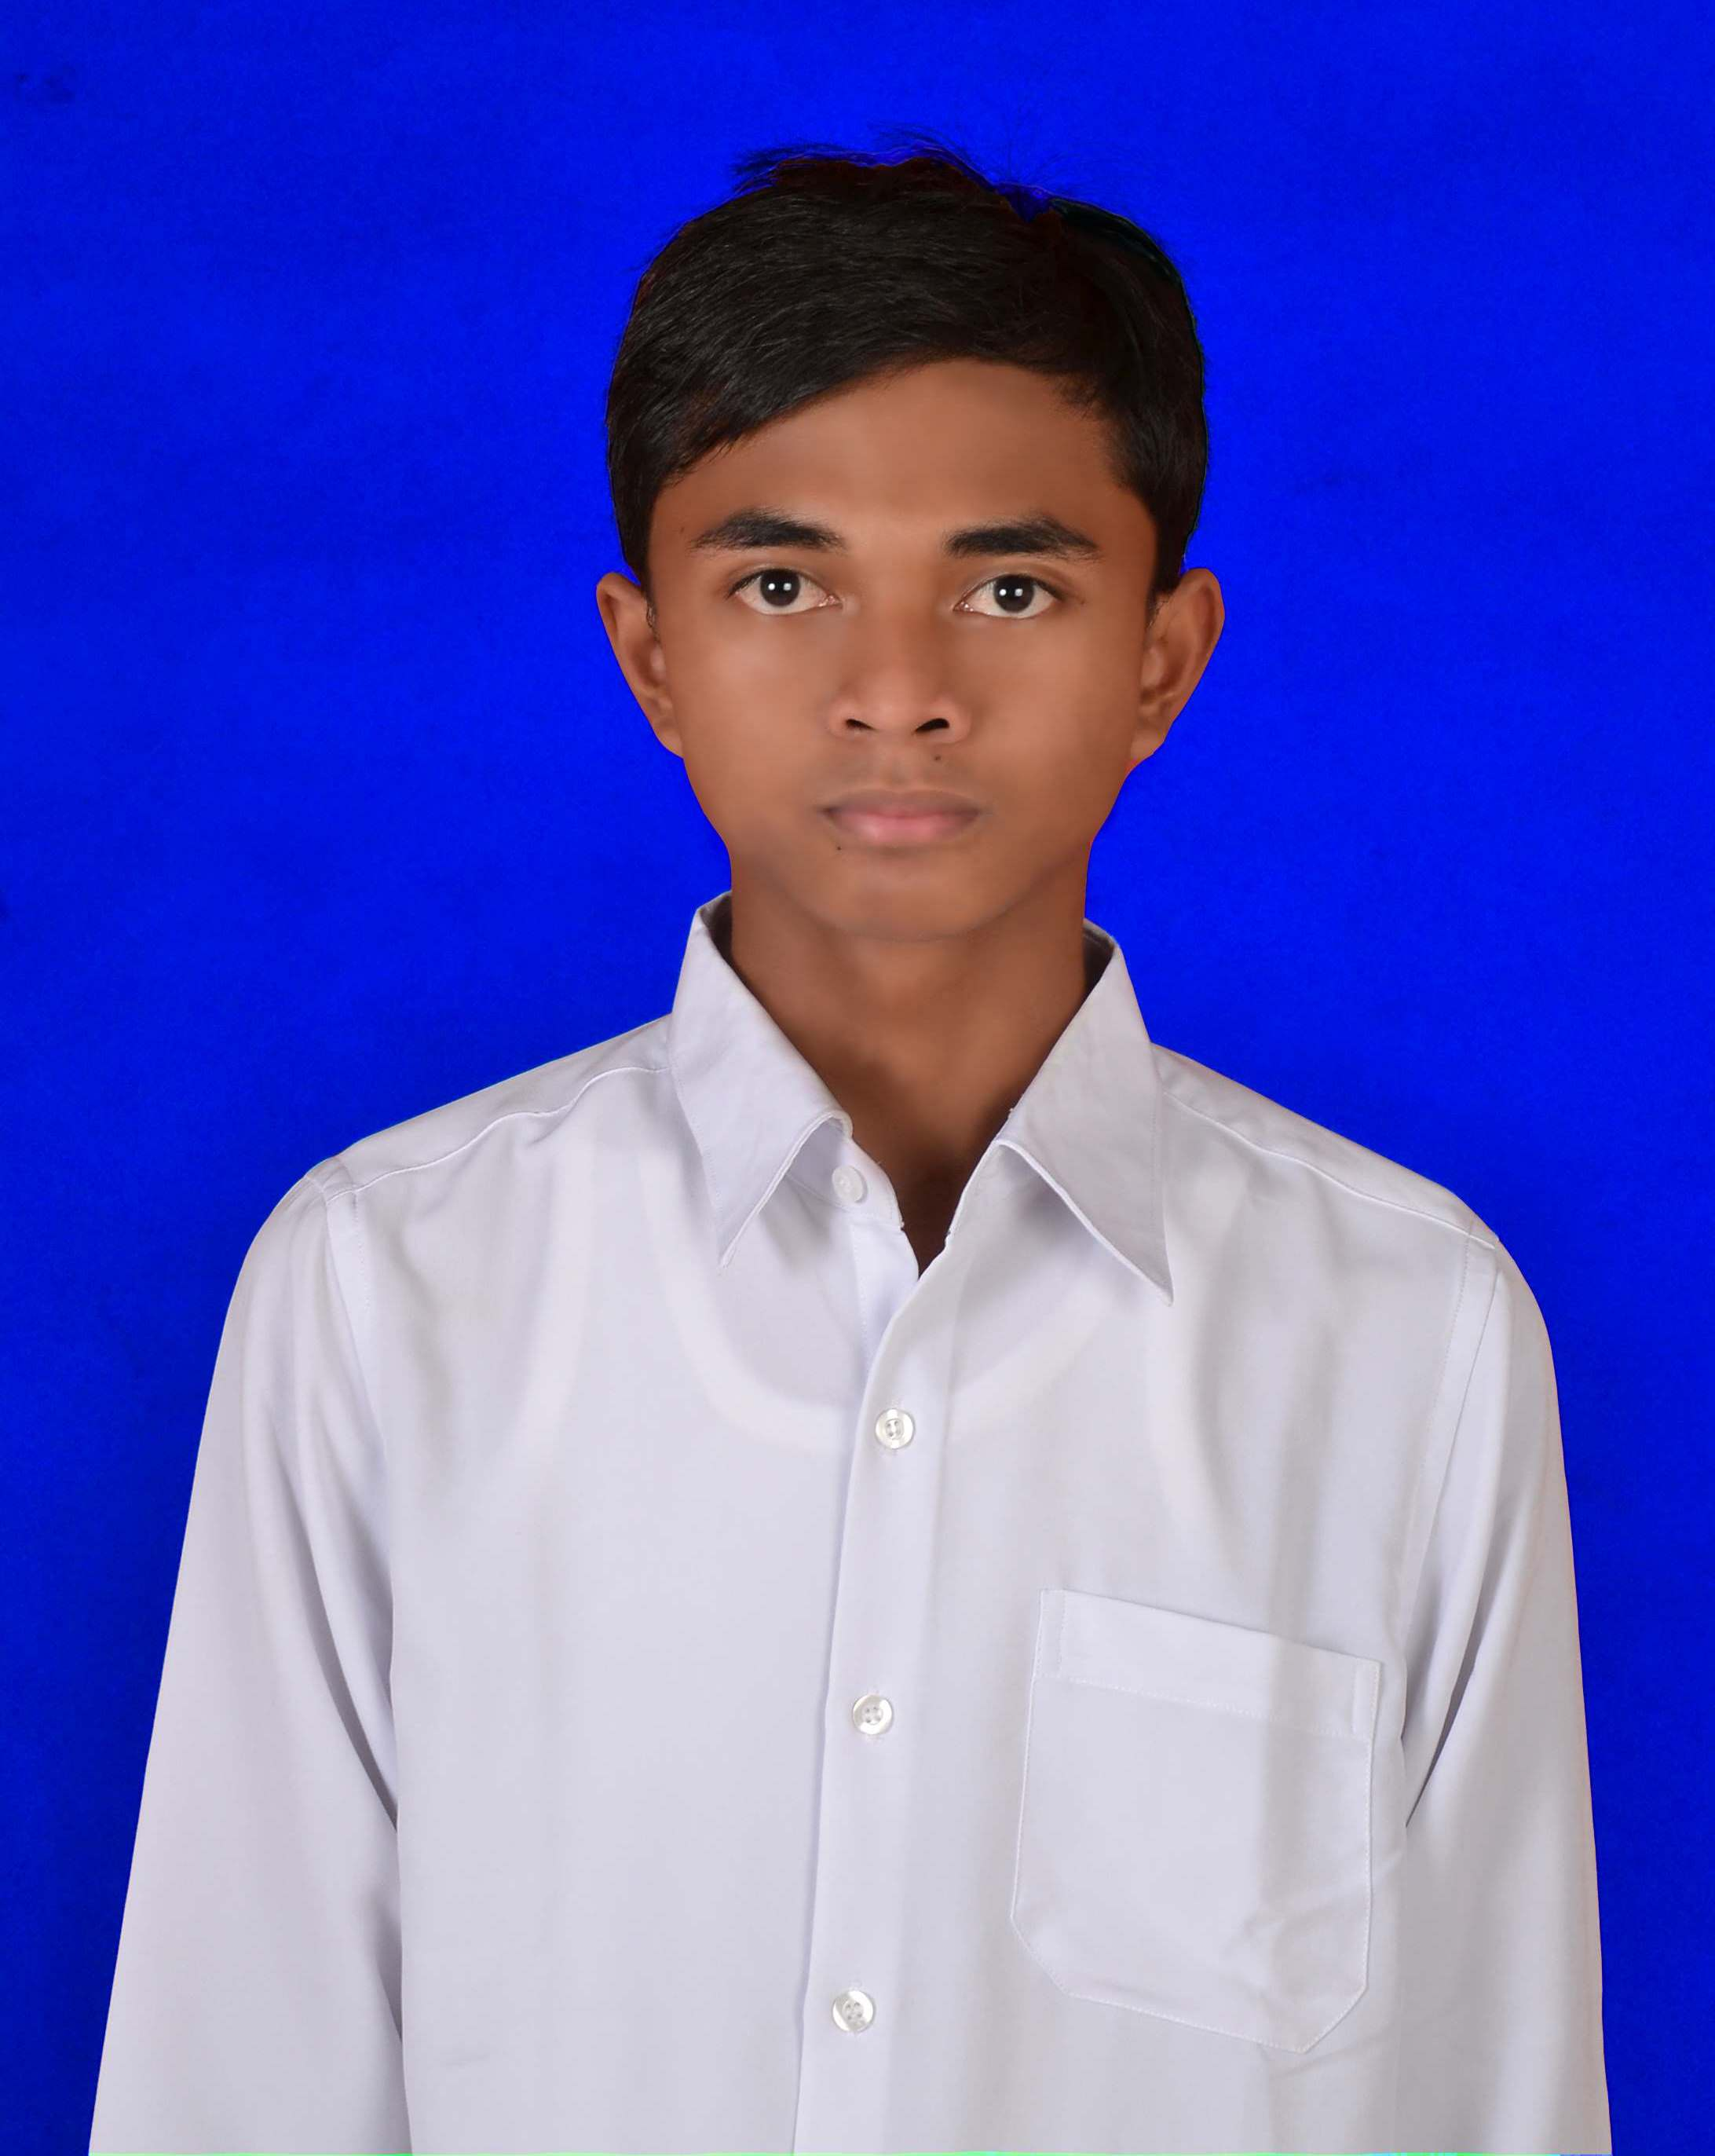
\includegraphics[width=0.29\textwidth]{Images/MFR.jpg}
		\end{wrapfigure}
		
		\textbf{Afif Ridho Kamal Putra}, akrab dipanggil Afif lahir pada tanggal 3 Oktober 1996 di Jakarta. Penulis merupakan seorang mahasiswa yang sedang menempuh studi di Departemen Informatika Institut Teknologi Sepuluh Nopember. Memiliki hobi antara lain makan dan bermain basket. Selama menempuh pendidikan di kampus, penulis juga aktif dalam organisasi kemahasiswaan, antara lain Staff Departemen Dalam Negeri Himpunan Mahasiswa Teknik Computer-Informatika pada tahun ke-2 dan Kepala Departemen Dalam Negeri Himpunan Mahasiswa Teknik Computer-Informatika pada tahun ke-3. Pernah menjadi staff Perlengkapan dan Transportasi Schematics tahun 2014 dan 2015. Selain itu penulis pernah menjadi asisten dosen dan asisten praktikum pada mata kuliah Sistem Operasi dan Jaringan Komputer.
\end{document}

\end{document} % YAY, WELCOME TO REAL WORD :)
